
%\newpage
\appendix


\section{Proof of Proposition 1}
\label{App:A}
%\begin{proposition}
%Considering only the arm elimination condition and $p=1$ the total regret till $T$ is upper bounded by $\E [R_{T}]\leq \sum\limits_{i\in A:\Delta_{i}\geq b}\bigg\lbrace\bigg(\dfrac{2^{1+4\rho_{a}}\rho_{a}^{2\rho_{a}}T^{1-\rho_{a}}}{\psi^{\rho_{a}}\Delta_{i}^{4\rho_{a}-1}}\bigg) + \bigg(\Delta_{i}+\dfrac{32\rho_{a}\log{(\psi T\dfrac{\Delta_{i}^{4}}{16\rho_{a}^{2}})}}{\Delta_{i}}\bigg)  +  \bigg(\dfrac{T^{1-\rho_{a}}\rho_{a}^{2\rho_{a}}2^{2\rho_{a}+\frac{3}{2}}}{\psi^{\rho_{a}}\Delta_{i}^{4\rho_{a} -1}} \bigg) \bigg \rbrace+\sum\limits_{i\in A:0\leq\Delta_{i}\leq b}\bigg(\dfrac{T^{1-\rho_{a}}\rho_{a}^{2\rho_{a}}2^{2\rho_{a}+\frac{3}{2}}}{\psi^{\rho_{a}}b^{4\rho_{a} -1}} \bigg) + max_{i:\Delta_{i}\leq b}\Delta_{i}T$ for all $b\geq\sqrt{\dfrac{e}{T}}$, where $\rho_{a}\in (0,1]$ is the arm elimination parameter, $\psi$ is the exploration regulatory factor, $p$ is the number of clusters and $T$ is the horizon.
%\end{proposition}

\begin{proof}

Let $p=1$ whereby we put all the arms in set $A$ into one cluster, that is we have one UCB-Improved running throughout. So, for each sub-optimal arm $a_{i}$, $m_{i}=\min{\lbrace m|\sqrt{\rho_{a}\epsilon_{m}} < \dfrac{\Delta_{i}}{2} \rbrace}$ be the first round when $\sqrt{\rho_{a}\epsilon_{m}} < \dfrac{\Delta_{i}}{2}$. Also in this proof, since the clusters are fixed, so throughout the rounds each $m_{i}$ is tied to a single arm. We also take $\rho_{a}\in (0,1]$ as a constant in this proof whereby in Corollary \ref{Result:Corollary:1} and \ref{Result:Corollary:2} we use the different definitions. The theoretical analysis remains same as we have always bounded the values of $\rho_{a}\in (0,1]$. Let $A^{'}=\lbrace i\in A: \Delta_{i} > b \rbrace$ and $A^{''}=\lbrace i\in A: 0 < \Delta_{i} \leq b \rbrace$.


\subsection*{Case a: \textit{Some sub-optimal arm $a_{i}$ is not eliminated in round $m_{i}$ or before and the optimal arm $a^{*}\in B_{m_{i}}$}}

 %In arm elimination condition, given the choice of confidence interval $c_{m_{i}}=\sqrt{\dfrac{\rho_{a}\log (\psi T\epsilon_{m_{i}}^{2})}{2 n_{m_{i}}}}$, we want to bound the probability of the event $\hat{r}_{i}+c_{m_{i}}\geq \hat{r}^{*}-c_{m_{i}}$. 
%In this proof we will consider $w_{s_{i}}=1$ and $\psi=1$. 
%Later, we will discuss how different values of $w_{s_{i}}$ actually effects the regret bound.
%with a more tighter event of $ \hat{r}_{i} + \sqrt{w_{s_{i}}}c_{m} \leq \hat{r}^{*} - \sqrt{w_{s_{i}}}c_{m}$ which will result in faster elimination of arms within a cluster, given the choice of $c_{m}$ and $w_{s_{i}}$.
%Now, $c_{m_{i}}=\sqrt{\dfrac{\rho_{a}\log (\psi T\epsilon_{m_{i}}^{2})}{2 n_{m_{i}}}}$.
  
	Following the steps of Theorem \ref{Result:Theorem:1} Case $a1$, an arbitrary sub-optimal arm $a_{i}\in A^{'}$ can get eliminated only when the event,
	\begin{align}
	\hat{r}_{i}  \le r_{i} + c_{m_{i}} \text{ and } 
 	\hat{r}^{*}\geq  r^{*} - c_{m_{i}}
	\end{align}
	
	takes place. So to bound the regret we need to bound the probability of the complementary event of these two conditions.
  
  Putting the value of $n_{m_{i}}=\dfrac{2\log{(\psi T\epsilon_{m_{i}}^{2})}}{\epsilon_{m_{i}}}$ in $c_{m_{i}}$,
  $c_{m_{i}}=\sqrt{\dfrac{\rho_{a}\epsilon_{m_{i}}\log (\psi T\epsilon_{m_{i}}^{2})}{2*2 \log(\psi T\epsilon_{m_{i}}^{2})}}=\dfrac{\sqrt{\rho_{a}\epsilon_{m_{i}}}}{2} = \sqrt{\rho_{a}\epsilon_{m_{i}+1}} < \dfrac{\Delta_{i}}{4} $, as $\rho_{a}\in (0,1]$.
%\leq\dfrac{\epsilon_{m}\sqrt{\ell_{m}}}{2\sqrt{w\ell_{m}}}\leq \dfrac{\epsilon_{m}}{2\sqrt{w}}$.
%  But in $\xi_{1}$, $\ell_{m}=2^{m}$.
%  Hence, $c\leq \dfrac{\epsilon_{m} 2^{m/2}}{4}$.
  
  Again, for $a_{i} \in A^{'}$, 
  \begin{align*}
\hat{r}_{i} + c_{m_{i}}&\leq r_{i} + 2c_{m_{i}} \\
&= \hat{r}_{i} + 4c_{m_{i}} - 2c_{m_{i}} \\
 &< r_{i} + \Delta_{i} - 2c_{m_{i}}\\
 &= r^{*} -2c_{m_{i}} \\
 &\leq \hat{r}^{*} - c_{m_{i}}
  \end{align*}

%% \hspace*{14em}$= \hat{r}_{i}-\sqrt{\epsilon_{m}} + 2c_{m} +\sqrt{\epsilon_{m}}$
% \hspace*{14em}$= r_{i} + 5\dfrac{\sqrt{\epsilon_{m}}}{\sqrt{w_{s_{i}}}} - 2\sqrt{w_{s_{i}}}c_{m}$
%  \hspace*{4em}
%  But, $\epsilon_{m}=\dfrac{\hat{\Delta}_{s,m}}{\ell_{m}}$, where $\hat{\Delta}_{s,m}=\max_{i\in B_{m}}{\hat{r}_{i}}-\min_{j\in B_{m}}{\hat{r}_{j}},i\neq j$ and $\ell_{m}$ is increased after every round.
%  \hspace*{4em}$\leq \hat{r}_{i} + \epsilon_{m} 2^{(m-4)/2} - 2c$
  Hence, we get that as soon as $\sqrt{\rho_{a}\epsilon_{m_{i}}}<\dfrac{\Delta_{i}}{2}$, $a_{i}$ gets eliminated.
%  So, $\hat{r}_{i}+c_{m}\leq \hat{r}_{i}+2c_{m}\leq r_{i} + \Delta_{i} - 2\sqrt{w_{s_{i}}}c_{m}\leq r^{*} - 2\sqrt{w_{s_{i}}}c_{m}$
%\leq \hat{r}^{*} - \sqrt{w}c_{m}
%  $\Rightarrow\hat{r}_{i}+c_{m}\leq \hat{r}_{i} - \sqrt{w}c_{m}  \leq r^{*} - \sqrt{w}c_{m}$
%  $\Rightarrow \hat{r}_{i} \leq {r}^{*} - 2\sqrt{w_{s_{i}}}c_{m} - 2c_{m} \leq \hat{r}^{*} - 2\sqrt{w_{s_{i}}}c_{m}$
% So, we need to bound the probability of the event of $\hat{r}_{i}+c_{m_{i}}\geq \hat{r}^{*}-c_{m_{i}}$.
%given that $\sqrt{\rho_{a}\epsilon_{m_{i}}}<\dfrac{\Delta_{i}}{2}$ becomes true for arm $a_{i}$ on or before $m_{i}$-th round with $c_{m_{i}}=\sqrt{\dfrac{\rho_{a}\log (\psi T\epsilon_{m_{i}}^{2})}{2 n_{m_{i}}}}$.
%  $\Rightarrow \hat{r}_{i}+2c_{m}\leq \hat{r}_{i} + 2\sqrt{w}c_{m} \leq \hat{r}^{*}$
%  $\Rightarrow \hat{r}_{i} + \sqrt{w}c_{m} \leq \hat{r}^{*} - \sqrt{w}c_{m}$
%  $\Rightarrow\hat{r}_{i}+c_{m}\sqrt{\dfrac{w\ell_{m}}{\epsilon_{m}}} \leq \hat{r}^{*}-c_{m}\sqrt{\dfrac{w\ell_{m}}{\epsilon_{m}}} $, as $c_{m}\sqrt{\dfrac{w\ell_{m}}{\epsilon_{m}}} > 0$

%\begin{proof} of Proposition 2:
% 
%Now, we can bound $\hat{r}_{i}+c_{m}\leq \hat{r}^{*}-c_{m}$ given that $\sqrt{\epsilon_{m}}<\dfrac{\Delta_{i}}{2}$ for some arm $a_{i}\in s_{i}$. 
%So, we need to bound the probability,
%	\begin{align*}
%	\mathbb{P}\lbrace\hat{r}^{*}\leq r^{*} - c_{m_{i}}\rbrace\leq U_{m}\text{, where $U_{m}$ is an  arbitrary upper bound.}
%	\end{align*}
 
%, for a fixed $n_{s_{i}}$.
%\mathbb{P}\lbrace\hat{r}^{*}\leq r^{*} - c_{m}\rbrace\leq
 
%Here, we guarantee that only if $\hat{r}^{*}\leq r^{*} - c_{m}\sqrt{\dfrac{w\ell_{m}}{\epsilon_{m}}}$ or $\hat{r}_{i}\geq r_{i} + c_{m}\sqrt{\dfrac{w\ell_{m}}{\epsilon_{m}}}$ then only arm will not be deleted. This is a more aggressive arm elimination condition than simply looking at $\hat{r}^{*}\leq r^{*} - c_{m}$ or $\hat{r}_{i}\geq r_{i} + c_{m}$ because we are exploring much carefully by dividing the larger problem into sub-problems.
% 
Applying Chernoff-Hoeffding bound and considering independence of events,
  \begin{align*}
\mathbb{P}\lbrace\hat{r}^{*}&\leq r^{*} - c_{m_{i}}\rbrace\leq exp(-2c_{m_{i}}^{2}n_{m_{i}})\\
&\leq exp(-2 * \dfrac{\rho_{a}\log (\psi T\epsilon_{m_{i}}^{2})}{2 n_{m_{i}}} *n_{m_{i}})\\
&\leq \dfrac{1}{(\psi T\epsilon_{m_{i}}^{2})^{\rho_{a}}}   
  \end{align*}
 
%$\leq \bigg(\dfrac{1}{4\psi T\epsilon_{m}^{2}}\bigg)^{D}$, as $\ell_{m}-1\leq D$
% \hspace*{2em}
 
Similarly, $\mathbb{P}\lbrace\hat{r}_{i}\geq r_{i} + c_{m_{i}}\rbrace\leq \dfrac{1}{(\psi  T\epsilon_{m_{i}}^{2})^{\rho_{a}}}$
 
Summing, the two up, the probability that a sub-optimal arm $a_{i}$ is not eliminated on or before $m_{i}$-th round is  $\bigg(\dfrac{2}{(\psi T\epsilon_{m_{i}}^{2})^{\rho_{a}}}\bigg)$. 
 
Summing up over all arms in $A$ and bounding trivially by $T\Delta_{i}$, we obtain
   \begin{align*}
\sum_{i\in A^{'}}\bigg(\dfrac{2T\Delta_{i}}{(\psi T\epsilon_{m_{i}}^{2})^{\rho_{a}}}\bigg)
&\leq\sum_{i\in A^{'}}\bigg(\dfrac{2T\Delta_{i}}{(\psi T\dfrac{\Delta_{i}^{4}}{16\rho_{a}^{2}})^{\rho_{a}}}\bigg)\\
&\leq \sum_{i\in A^{'}}\bigg(\dfrac{2^{1+4\rho_{a}}T^{1-\rho_{a}}\rho_{a}^{2\rho_{a}}\Delta_{i}}{\psi^{\rho_{a}}\Delta_{i}^{4\rho_{a}}}\bigg)\\
&\leq \sum_{i\in A^{'}}\bigg(\dfrac{2^{1+4\rho_{a}}\rho_{a}^{2\rho_{a}}T^{1-\rho_{a}}}{\psi^{\rho_{a}}\Delta_{i}^{4\rho_{a}-1}}\bigg)\\   
& =\sum_{i\in A^{'}}\bigg(\dfrac{C_{1}(\rho_{a})T^{1-\rho_{a}}}{\Delta_{i}^{4\rho_{a}-1}}\bigg) \text{, where } C_1(x) = \frac{2^{1+4x}x^{2x}}{\psi^{x}}
   \end{align*}

%$C_1(x) = \frac{2^{1+4x}x^{2x}}{\psi^{x}}$ and $C_2(x) = \frac{2^{2x+\frac{3}{2}}x^{2x}}{\psi^{x}}$

% 
%Summing up over all arms in $A$ and bounding trivially by $T\Delta_{i}$,
%%\sum_{i\in A}\bigg(\dfrac{2}{T\epsilon_{m_{i}}^{2}}\bigg)\leq
% \hspace*{4em} $\sum_{i\in A}\bigg(\dfrac{2*4T\Delta_{i}}{T\epsilon_{m_{i}}\dfrac{\Delta_{i}}{2}^{2}}\bigg)\leq \sum_{i\in A}\bigg(\dfrac{8}{\epsilon_{m_{i}}\Delta_{i}}\bigg)\leq \sum_{i\in A}\bigg(\dfrac{32}{\Delta_{i}^{3}}\bigg)$


%\textbf{Case b1:} Either an arm $a_{i}$ is eliminated in round $m_{i}$ or before or else there is no optimal arm $a^{*}\in B_{m_{i}}$. 

\subsection*{Case b: \textit{Either an arm $a_{i}$ is eliminated in round $m_{i}$ or before or else there is no optimal arm $a^{*}\in B_{m_{i}}$ }}

\subsubsection*{Case b1: \textit{$a^{*}\in B_{m_{i}}$ and $a_{i}\in A^{'}$ is  eliminated on or before $m_{i}$ } }

 Since we are eliminating a sub-optimal arm $a_{i}$ on or before round $m_{i}$, it is pulled no longer than, 
 \begin{align*}
 n_{m_{i}}=\bigg\lceil\dfrac{2\log{(\psi T\epsilon_{m_{i}}^{2})}}{\epsilon_{m_{i}}}\bigg\rceil
 \end{align*}
%\hspace*{4em}
%%$, since $\sqrt{\rho_{a}\epsilon_{m_{i}}}\leq\dfrac{\Delta_{i}}{2}
So, the total contribution of $a_{i}$  till round $m_{i}$ is given by, 
\begin{align*}
&\Delta_{i}\bigg\lceil\dfrac{2\log{(\psi T\epsilon_{m_{i}}^{2})}}{\epsilon_{m_{i}}}\bigg\rceil\\
&\leq\Delta_{i}\bigg\lceil\dfrac{2\log{(\psi T(\dfrac{\Delta_{i}}{2\sqrt{\rho_{a}})^{4})}}}{(\dfrac{\Delta_{i}}{2\sqrt{\rho_{a}}})^{2}}\bigg\rceil \text{, since } \sqrt{\rho_{a}\epsilon_{m_{i}}}\leq\dfrac{\Delta_{i}}{2}\\
&\leq\Delta_{i}\bigg(1+\dfrac{32\rho_{a}\log{(\psi T(\dfrac{\Delta_{i}}{2\sqrt{\rho_{a}}})^{4})}}{\Delta_{i}^{2}}\bigg)
\\
&\leq\Delta_{i}\bigg(1+\dfrac{32\rho_{a}\log{(\psi T\dfrac{\Delta_{i}^{4}}{16\rho_{a}^{2}})}}{\Delta_{i}^{2}}\bigg)
\end{align*} 
 
Summing over all arms in $A^{'}$ the total regret is given by, 
\begin{align*}
\sum_{i\in A^{'}}\Delta_{i}\bigg(1+\dfrac{32\rho_{a}\log{(\psi T\dfrac{\Delta_{i}^{4}}{16\rho_{a}^{2}}})}{\Delta_{i}^{2}}\bigg)
\end{align*}

\subsubsection*{Case b2: \textit{Optimal arm $a^{*}$ is eliminated by a sub-optimal arm  }}


	Firstly, if conditions of Cases $a-b1$ holds then the optimal arm $a^{*}$ will not be eliminated in round $m=m_{*}$ or it will lead to the contradiction that $r_{i}>r^{*}$. In any round $m_{*}$, if the optimal arm $a^{*}$ gets eliminated then for any round from $1$ to $m_{j}$ all arms $a_{j}$ such that $\sqrt{\rho_{a}\epsilon_{m}}<\dfrac{\Delta_{j}}{2}$ were eliminated according to assumption in Case $a$. Let, the arms surviving till $m_{*}$ round be denoted by $A^{'}$. This leaves any arm $a_{b}$ such that $\sqrt{\rho_{a}\epsilon_{m}}\geq\dfrac{\Delta_{b}}{2}$ to still survive and eliminate arm $a^{*}$ in round $m_{*}$. Let, such arms that survive $a^{*}$ belong to $A^{''}$. Also maximal regret per step after eliminating $a^{*}$ is the maximal $\Delta_{j}$ among the remaining arms $a_{j}$ with $m_{j}\geq m_{*}$.  Let $m_{b}$ be the round when $\sqrt{\rho_{a}\epsilon_{m}}<\dfrac{\Delta_{b}}{2}$ that is $m_{b}=\min\lbrace m|\sqrt{\rho_{a}\epsilon_{m}}<\dfrac{\Delta_{b}}{2}\rbrace$. Hence, the maximal regret after eliminating the arm $a^{*}$ is upper bounded by, 
\begin{align*}
&\sum_{m_{*}=0}^{max_{j\in A^{'}}m_{j}}\sum_{i\in A^{''}:m_{i}>m_{*}}\bigg(\dfrac{2}{(\psi  T\epsilon_{m_{*}}^{2})^{\rho_{a}}} \bigg).T\max_{j\in A^{''}:m_{j}\geq m_{*}}{\Delta}_{j}\\
&\leq\sum_{m_{*}=0}^{max_{j\in A^{'}}m_{j}}\sum_{i\in A^{''}:m_{i}>m_{*}}\bigg(\dfrac{2}{(\psi  T\epsilon_{m_{*}}^{2})^{\rho_{a}}} \bigg).T.2\sqrt{\rho_{a}\epsilon_{m_{*}}}\\
&\leq\sum_{m_{*}=0}^{max_{j\in A^{'}}m_{j}}\sum_{i\in A^{''}:m_{i}>m_{*}}4\bigg(\dfrac{T^{1-\rho_{a}}}{\psi^{\rho_{a}}\epsilon_{m_{*}}^{2\rho_{a}-\frac{1}{2}}} \bigg)\\
&\leq\sum_{i\in A^{''}:m_{i}>m_{*}}\sum_{m_{*}=0}^{\min{\lbrace m_{i},m_{b}\rbrace}}\bigg(\dfrac{4T^{1-\rho_{a}}}{\psi^{\rho_{a}}2^{-(2\rho_{a}-\frac{1}{2})m_{*}}} \bigg)\\
&\leq\sum_{i\in A^{'}}\bigg(\dfrac{4T^{1-\rho_{a}}}{\psi^{\rho_{a}}2^{-(2\rho_{a}-\frac{1}{2})m_{*}}} \bigg)+\sum_{i\in A^{''}\setminus A^{'}}\bigg(\dfrac{4T^{1-\rho_{a}}}{\psi^{\rho_{a}}2^{-(2\rho_{a}-\frac{1}{2})m_{b}}} \bigg)\\
&\leq\sum_{i\in A^{'}}\bigg(\dfrac{4\rho_{a}^{2\rho_{a}}T^{1-\rho_{a}}*2^{2\rho_{a}-\frac{1}{2}}}{\psi^{\rho_{a}}\Delta_{i}^{4\rho_{a}-1}} \bigg)+\sum_{i\in A^{''}\setminus A^{'}}\bigg(\dfrac{4\rho_{a}^{2\rho_{a}}T^{1-\rho_{a}}*2^{2\rho_{a}-\frac{1}{2}}}{\psi^{\rho_{a}}b^{4\rho_{a}-1}} \bigg)\\
&\leq\sum_{i\in A^{'}}\bigg(\dfrac{T^{1-\rho_{a}}\rho_{a}^{2\rho_{a}}2^{2\rho_{a}+\frac{3}{2}}}{\psi^{\rho_{a}}\Delta_{i}^{4\rho_{a}-1}} \bigg)+\sum_{i\in A^{''}\setminus A^{'}}\bigg(\dfrac{T^{1-\rho_{a}}\rho_{a}^{2\rho_{a}}2^{2\rho_{a}+\frac{3}{2}}}{\psi^{\rho_{a}}b^{4\rho_{a}-1}} \bigg)\\
& = \sum_{i\in A^{'}}\bigg(\dfrac{ C_{2}(\rho_{a}) T^{1-\rho_{a}}}{\Delta_{i}^{4\rho_{a}-1}} \bigg)+\sum_{i\in A^{''}\setminus A^{'}}\bigg(\dfrac{C_{2(\rho_{a})}T^{1-\rho_{a}}}{b^{4\rho_{a}-1}} \bigg) \text{, where } C_2(x) = \frac{2^{2x+\frac{3}{2}}x^{2x}}{\psi^{x}}
\end{align*}

%\text{, since } \sqrt{\rho_{a}\epsilon_{m}}<\dfrac{\Delta_{i}}{2}

 
Summing up \textbf{Case a} and \textbf{Case b}, the total regret till round $m$ is given by,
\begin{align*}
 R_{T} \leq &\sum\limits_{i\in A:\Delta_{i} > b}\bigg\lbrace\bigg(\dfrac{C_{1}(\rho_{a})T^{1-\rho_{a}}}{\Delta_{i}^{4\rho_{a}-1}}\bigg) + \bigg(\Delta_{i}+\dfrac{32\rho_{a}\log{(\psi  T\dfrac{\Delta_{i}^{4}}{16\rho_{a}^{2}})}}{\Delta_{i}}\bigg)\\
&  +  \bigg(\dfrac{C_{2}(\rho_{a})T^{1-\rho_{a}}}{\Delta_{i}^{4\rho_{a} -1}} \bigg) \bigg \rbrace+\sum\limits_{i\in A:0\leq\Delta_{i}\leq b}\bigg(\dfrac{C_{2}(\rho_{a})T^{1-\rho_{a}}}{\psi^{\rho_{a}}b^{4\rho_{a} -1}} \bigg) + max_{i:\Delta_{i}\leq b}\Delta_{i}T
\end{align*}

% R_{T} \leq &\sum\limits_{i\in A:\Delta_{i}\geq b}\bigg\lbrace\bigg(\dfrac{2^{1+4\rho_{a}}\rho_{a}^{2\rho_{a}}T^{1-\rho_{a}}}{\psi^{\rho_{a}}\Delta_{i}^{4\rho_{a}-1}}\bigg) + \bigg(\Delta_{i}+\dfrac{32\rho_{a}\log{(\psi  T\dfrac{\Delta_{i}^{4}}{16\rho_{a}^{2}})}}{\Delta_{i}}\bigg)\\
%&  +  \bigg(\dfrac{T^{1-\rho_{a}}\rho_{a}^{2\rho_{a}}2^{2\rho_{a}+\frac{3}{2}}}{\psi^{\rho_{a}}\Delta_{i}^{4\rho_{a} -1}} \bigg) \bigg \rbrace+\sum\limits_{i\in A:0\leq\Delta_{i}\leq b}\bigg(\dfrac{T^{1-\rho_{a}}\rho_{a}^{2\rho_{a}}2^{2\rho_{a}+\frac{3}{2}}}{\psi^{\rho_{a}}b^{4\rho_{a} -1}} \bigg) + max_{i:\Delta_{i}\leq b}\Delta_{i}T
  
\end{proof}

\section{Proof of Proposition 2}
\label{App:B}

\begin{figure}
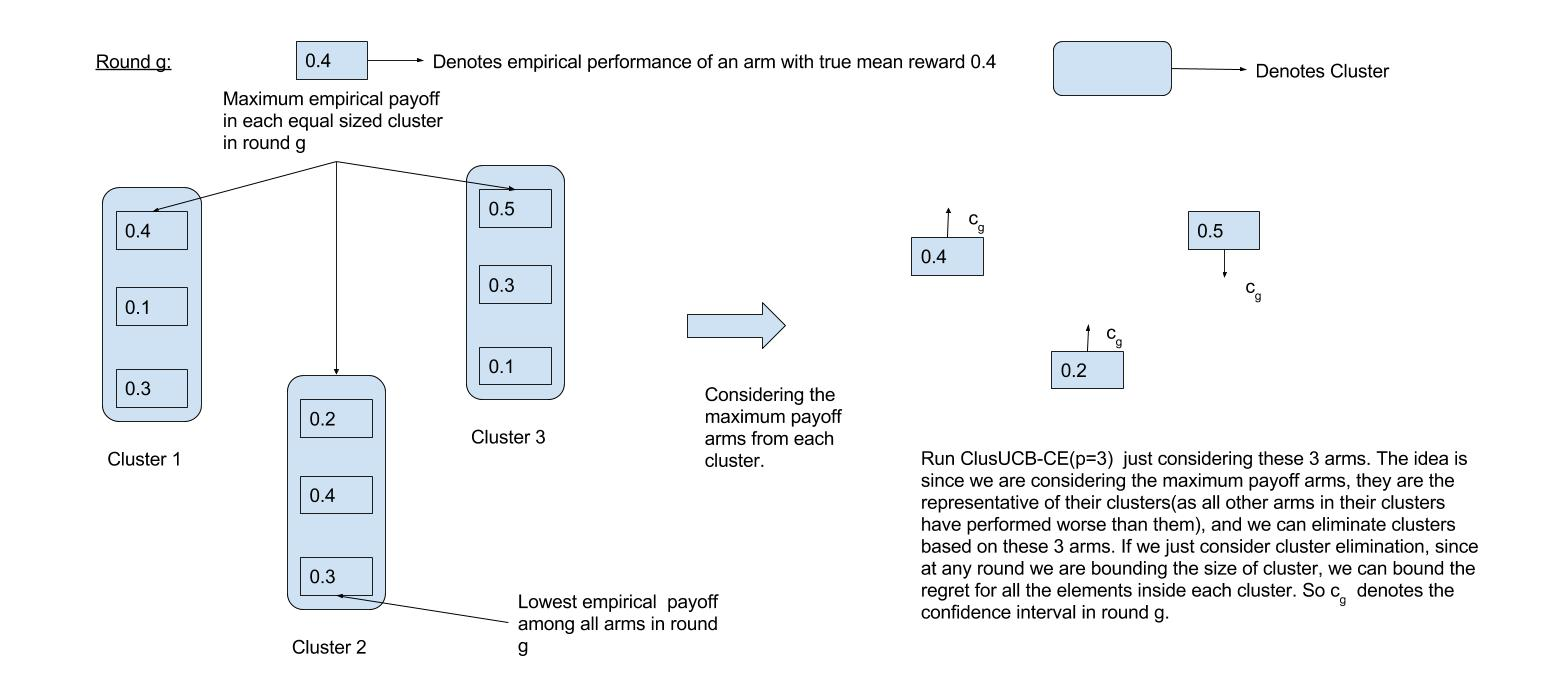
\includegraphics[scale=0.3]{img/diagCluster.jpg}
\caption{Cluster Elimination}
\label{Fig:ClusFig}
\end{figure}

%\begin{proposition}
%Considering only the cluster elimination condition and $p>1$, the total regret till $T$ is upper bounded by $\E [R_{T}]\leq \sum\limits_{i\in A:\Delta_{i}\geq b}\bigg\lbrace \bigg(\dfrac{2^{2+4\rho_{s}}\rho_{s}^{2\rho_{s}}T^{1-\rho_{s}}}{\psi^{\rho_{s}}\Delta_{i}^{4\rho_{s}-1}}\bigg) + \bigg(\Delta_{i}+\dfrac{32\rho_{s}\log{(\psi T\dfrac{\Delta_{i}^{4}}{16\rho_{s}^{2}})}}{\Delta_{i}}\bigg)  +  \bigg(\dfrac{T^{1-\rho_{s}}\rho_{s}^{2\rho_{s}}2^{2\rho_{s}+3}}{\psi^{\rho_{s}}\Delta_{i}^{4\rho_{s} -1}} \bigg)\bigg \rbrace +\sum\limits_{i\in A:0\leq\Delta_{i}\leq b}\bigg(\dfrac{T^{1-\rho_{s}}\rho_{s}^{2\rho_{s}}2^{2\rho_{s}+3}}{\psi^{\rho_{s}}b^{4\rho_{s} -1}} \bigg) + max_{i:\Delta_{i}\leq b}\Delta_{i}T$ for all $b\geq \sqrt{\dfrac{e}{T}}$, where $\rho_{s}\in (0,1]$ is the cluster elimination parameter, $\psi$ is the exploration regulatory factor, $p$ is the number of clusters and $T$ is the horizon.
%\end{proposition}

An illustrative diagram explaining Cluster Elimination is given in \textbf{Figure \ref{Fig:ClusFig}}. A slight modification to the algorithm allows us to do cluster elimination without any arm elimination. By taking $p>1$, removing the arm elimination condition, stopping when we are just left with one cluster and pulling the $max\lbrace \hat{r}_{i}\rbrace$, where $a_{i}\in B_{m}$ we can achieve this. We also take $\rho_{s}\in (0,1]$ as a constant in this proof whereby in Corollary \ref{Result:Corollary:1} and \ref{Result:Corollary:2} we use the different definitions. The theoretical analysis remains same as we have always bounded the values of $\rho_{s}\in (0,1]$(see Appendix \ref{App:E}). 
 

\begin{proof}
 A sketch of the proof is given below,

\begin{itemize}
\item Define $C_{g}$ as the active cluster set which contains the max payoff arm from all the clusters active in the $g$-th round. So, the maximum cardinality of $C_{g}$ is $p$ and also this is always a non-increasing set.
\item Now, the elements in $C_{g}$ which are the max-payoff arm from each cluster(if there are more than $1$ max-payoff arm in a cluster then choose randomly between them) are not fixed and hence like $B_{m}$ in proposition \ref{proofTheorem:Prop:1} cannot be tied to an arm $a_{i}$ throughout the rounds. For this purpose the $i$-th element in $C_{g}$ we tie to a cluster, that is $a_{\max_{s_{k}}}\in C_{g}$ is the max payoff arm in the cluster $s_{k}$ if the cluster $s_{k}$ still surviving in round $g$ and call $a_{\max_{s_{k}}}$ as a cluster arm. 
\item Define $g$-th round(like in proposition \ref{proofTheorem:Prop:1}) as the same way as the $m$-th round signifying the first/minimum round when a cluster gets eliminated.
%\item Let in the $g$-th round $C_{g}$ be the set which contains all the max payoff arms from each cluster.
\item For regret bound proof according to proposition \ref{proofTheorem:Prop:1}, consider only this $C_{g}$ and proof following the same way as in proposition \ref{proofTheorem:Prop:1} with some changes. In any round $g$, atleast one of these $5$ events must occur:-
\begin{itemize}
\item \textbf{Case a1:} $a^{*}\in C_{g}$ and bound the regret that a sub-optimal cluster arm $a_{\max_{s_{k}}}\in C_{g}$ does not get eliminated on or before $g_{s_{k}}$-th round.
\item \textbf{Case a2:} $a^{*}\notin C_{g}$ and bound the regret that a sub-optimal cluster arm $a_{\max_{s_{k}}}$ does not get eliminated on or before $a_{max_{s^{*}}}\in C_{g}$, such that $a_{\max_{s^{*}}},a^{*}\in s^{*}$ and $a_{\max_{s^{*}}}\neq a^{*}$. So, $a^{*}$ survives by this condition.
\item \textbf{Case b1:} Cluster arm $a_{s_{k}}$ gets eliminated on $g_{s_{k}}$-th round(or before) with $a^{*}$ still in $B_{g_{s_{k}}}$ and calculate the regret for the arm pulls for all arms in cluster $s_{k}$(clusters are fixed).
\item \textbf{Case b2:} $a^{*}\in C_{g}$ and $s^{*}$ gets eliminated by another sub-optimal cluster arm and bound this regret.
\item \textbf{Case b3:} $a^{*}\notin C_{g}$ and $s^{*}$ gets eliminated by another sub-optimal cluster arm  and bound this regret.
\end{itemize}
For bounding the regret we use Chernoff-Hoeffding bound and use it on the current set of cluster arms $a_{max_{s_{k}}}\in C_{g},\forall s_{k}\in S$. This will work because of the algorithm, we are pulling all the  surviving arms equal number of times in each round and applying the same confidence interval for cluster elimination to all of the elements of $C_{g}$ and also we fix the clusters from beginning of the rounds.
%Hence, $C_{g}$ actually behaves like the set $B_{m}$ in proposition $5$ but contains just the max payoff arm from each cluster.
\item Introduce a constant $\rho_{s}\in (0,1]$ for cluster elimination to mimic the arm elimination condition in proposition \ref{proofTheorem:Prop:1}, but with the condition that whenever $\sqrt{\rho_{s}\epsilon_{g_{s_{k}}}} <  \dfrac{\Delta_{a_{\max_{s_{k}}}}}{2}, a_{\max_{s_{k}}}\in C_{g}$, then the cluster $s_{k}$(where 
$\hat{r}_{a_{\max_{s_{k}}}}$ is the max payoff) gets eliminated. Because of the algorithm, we are guaranteed that the  maximum size of the cluster in the $g$-th round is $\ell=\bigg\lceil \dfrac{K}{p}\bigg\rceil$.
\end{itemize}

Let $C_{g}=\lbrace \hat{r}_{\max_{s_{k}}}| \forall s_{k}\in S \rbrace$, that is let $C_{g}$ be the set of all arms which has the maximum estimated payoff in their respective clusters in the $g$-th round.

Let, for each sub-optimal cluster arm $a_{\max_{s_{k}}}\in C_{g_{s_{k}}}$, $g_{s_{k}}=\min{\lbrace g|\sqrt{\rho_{s}\epsilon_{g}}leq \dfrac{\Delta_{a_{\max_{s_{k}}}}}{2} \rbrace}$. So, $g_{s_{k}}$ be the first round when $\sqrt{\rho_{s}\epsilon_{g_{s_{k}}}} < \dfrac{\Delta_{a_{\max_{s_{k}}}}}{2}$ where $a_{\max_{s_{k}}}\in C_{g_{s_{k}}}$ is the maximum payoff arm in cluster $s_{k}$ and then $s_{k}$ gets eliminated. Here, $a_{\max_{s_{k}}}$ is called cluster arm. We will also consider for Case $a1,b1 $ and $b2$  that $\max \hat{r}_{i}\in C_{g_{s_{k}}}$ is $a^{*}$ and it has not still been eliminated. For case $a2$ and $b2$ we will consider $a^{*}$ not in $C_{g_{s_{k}}}$. Here, $A_{{s_{k}}}$ denotes the arm set in the cluster $s_{k}$. So, for cluster elimination we will only be considering the arms in $C_{g_{s_{k}}}$ called cluster arms, and follow the proof of proposition \ref{proofTheorem:Prop:1}. Let $A_{s_{k}}^{'}=\lbrace i\in A_{s_{k}}: \Delta_{i}> b\rbrace$, $A_{s_{k}}^{''}=\lbrace i\in A_{s_{k}}: 0 < \Delta_{i} \leq b\rbrace$, $A^{'}=\lbrace i\in A: \Delta_{i}> b\rbrace$ and $A^{''}=\lbrace i\in A: 0 < \Delta_{i} \leq b\rbrace$.

%The parameter $\rho_{s}$ is introduced just to make sure that the cluster elimination is a more aggressive elimination than arm elimination.
\subsection*{Case a: \textit{ Some sub-optimal cluster arm $a_{max_{s_{k}}}$ is not eliminated in round $g_{s_{k}}$ or before }}
\subsubsection*{Case a1: \textit{ Some sub-optimal cluster arm $a_{max_{s_{k}}}$ is not eliminated in round $g_{s_{k}}$ or before and the optimal cluster arm $a^{*}\in C_{g_{s_{k}}} \subset B_{m}$ }}

	In arm elimination condition, given the choice of confidence interval $c_{g_{s_{k}}}=\sqrt{\dfrac{\rho_{s} \log (\psi T\epsilon_{g_{s_{k}}}^{2})}{2 n_{g_{s_{k}}}}}$, we want to bound the probability of the event $\hat{r}_{s_{k}}+c_{g_{s_{k}}}\geq \hat{r}^{*}-c_{g_{s_{k}}}$.
%with a more tighter event of $ \hat{r}_{i} + \sqrt{w_{s_{k}}}c_{m} \leq \hat{r}^{*} - \sqrt{w_{s_{k}}}c_{m}$ which will result in faster elimination of arms within a cluster, given the choice of $c_{m}$ and $w_{s_{k}}$.
  %Now, $c_{g_{s_{k}}}=\sqrt{\dfrac{\rho_{s} \log (\psi T\epsilon_{g_{s_{k}}}^{2})}{2 n_{g_{s_{k}}}}}$, where $0 < \rho_{s}\leq 1$.
  Putting the value of $n_{g_{s_{k}}}=\dfrac{2\log{(\psi T\epsilon_{g_{s_{k}}}^{2})}}{\epsilon_{g_{s_{k}}}}$ in $c_{g_{s_{k}}}$ we get,
  \begin{align*}
  c_{g_{s_{k}}}= & \sqrt{\dfrac{\rho_{s}*\epsilon_{g_{s_{k}}}\log (\psi  T\epsilon_{g_{s_{k}}}^{2})}{2*2 \log(\psi T\epsilon_{g_{s_{k}}}^{2})}}\\
  &=\sqrt{\dfrac{\rho_{s}\epsilon_{g_{s_{k}}}}{2}}\\
  &=\sqrt{\rho_{s}\epsilon_{g_{s_{k}}+1}} < \dfrac{\sqrt{\rho_{s}}\Delta_{a_{\max_{s_{k}}}}}{4} < \dfrac{\Delta_{a_{\max_{s_{k}}}}}{4}
  \end{align*}
%  $c_{g_{s_{k}}}=\sqrt{\dfrac{\rho_{s}*\epsilon_{g_{s_{k}}}\log (\psi T\epsilon_{g_{s_{k}}}^{2})}{2*2 \log(\psi T\epsilon_{g_{s_{k}}}^{2})}}=\sqrt{\dfrac{\rho_{s}\epsilon_{g_{s_{k}}}}{2}} = \sqrt{\rho_{s}\epsilon_{g_{s_{k}}+1}} < \dfrac{\sqrt{\rho_{s}}\Delta_{a_{max_{s_{k}}}}}{4} < \dfrac{\Delta_{a_{max_{s_{k}}}}}{4} $

  Again, for $a_{\max_{s_{k}}} \in C_{g_{s_{k}}}$, 
  \begin{align*}
  \hat{r}_{a_{\max_{s_{k}}}} + c_{g_{s_{k}}}\leq r_{a_{\max_{s_{k}}}} + 2c_{g_{s_{k}}} &= \hat{r}_{a_{\max_{s_{k}}}} + 4c_{g_{k}} - 2c_{g_{s_{k}}}\\
  &< r_{a_{\max_{s_{k}}}} + \Delta_{a_{\max_{s_{k}}}} - 2c_{g_{s_{k}}}\\
  &= r^{*} -2c_{g_{s_{k}}}\\
  &\leq \hat{r}^{*} - c_{g_{s_{k}}}
  \end{align*}
   
 	Hence, we get that as soon as $\sqrt{\rho_{s}\epsilon_{g_{s_{k}}}}<\dfrac{\Delta_{a_{max_{s_{k}}}}}{2}$, 
 	$a_{max_{s_{k}}}\in C_{g_{s_{k}}}$ gets eliminated.
%  So, $\hat{r}_{i}+c_{m}\leq \hat{r}_{i}+2c_{m}\leq r_{i} + \Delta_{i} - 2\sqrt{w_{s_{k}}}c_{m}\leq r^{*} - 2\sqrt{w_{s_{k}}}c_{m}$
%\leq \hat{r}^{*} - \sqrt{w}c_{m}
%  $\Rightarrow\hat{r}_{i}+c_{m}\leq \hat{r}_{i} - \sqrt{w}c_{m}  \leq r^{*} - \sqrt{w}c_{m}$
%  $\Rightarrow \hat{r}_{i} \leq {r}^{*} - 2\sqrt{w_{s_{k}}}c_{m} - 2c_{m} \leq \hat{r}^{*} - 2\sqrt{w_{s_{k}}}c_{m}$
  So, we need to bound the probability of the event of $\hat{r}_{a_{max_{s_{k}}}}+c_{g_{s_{k}}}\geq \hat{r}^{*}-c_{g_{s_{k}}}$.
  %given that $\sqrt{\rho_{s}\epsilon_{g_{s_{k}}}}<\dfrac{\Delta_{a_{max_{s_{k}}}}}{2}$ becomes true for some arm $a_{max_{s_{k}}}\in C_{g_{s_{k}}}$ after the $g$-th round and $c_{g_{s_{k}}}=\sqrt{\dfrac{\rho_{s} \log (\psi T\epsilon_{g_{s_{k}}}^{2})}{2 n_{g_{s_{k}}}}}$.
%  $\Rightarrow \hat{r}_{i}+2c_{m}\leq \hat{r}_{i} + 2\sqrt{w}c_{m} \leq \hat{r}^{*}$
%  $\Rightarrow \hat{r}_{i} + \sqrt{w}c_{m} \leq \hat{r}^{*} - \sqrt{w}c_{m}$
%  $\Rightarrow\hat{r}_{i}+c_{m}\sqrt{\dfrac{w\ell_{m}}{\epsilon_{m}}} \leq \hat{r}^{*}-c_{m}\sqrt{\dfrac{w\ell_{m}}{\epsilon_{m}}} $, as $c_{m}\sqrt{\dfrac{w\ell_{m}}{\epsilon_{m}}} > 0$

%\begin{proof} of Proposition 2:
% 
%Now, we can bound $\hat{r}_{i}+c_{m}\leq \hat{r}^{*}-c_{m}$ given that $\sqrt{\epsilon_{m}}<\dfrac{\Delta_{i}}{2}$ for some arm $a_{i}\in s_{k}$. 
%	So, we need to bound the probability,
%	\begin{align*}
%	&\mathbb{P}\lbrace\hat{r}^{*}\leq r^{*} - c_{g_{s_{k}}}\rbrace\leq U_{g}\text{, where $U_{g}$ is an  arbitrary upper bound.}
%	\end{align*}

	Applying Chernoff-Hoeffding bound and considering independence of events,
 
 \begin{align*}
 \mathbb{P}\bigg\lbrace\hat{r}^{*} \leq r^{*} - c_{g_{s_{k}}}\bigg\rbrace&\leq exp(-2c_{g_{s_{k}}}^{2}n_{g_{s_{k}}})\\
 &\leq exp(-2 * \dfrac{\rho_{s}\log ( \psi T\epsilon_{g_{s_{k}}}^{2})}{2 n_{g_{s_{k}}}} *n_{g_{s_{k}}})\\
 &\leq \dfrac{1}{(\psi T\epsilon_{g_{k}}^{2})^{\rho_{s}}}
 \end{align*}
% \hspace*{0em} $\mathbb{P}\lbrace\hat{r}^{*}\leq r^{*} - c_{g_{s_{k}}}\rbrace\leq exp(-2c_{g_{s_{k}}}^{2}n_{g_{s_{k}}})$
% \hspace*{8em} $\leq exp(-2 * \dfrac{\rho_{s}\log ( \psi T\epsilon_{g_{s_{k}}}^{2})}{2 n_{g_{s_{k}}}} *n_{g_{s_{k}}})$
% \hspace*{8em} $\leq \dfrac{1}{(\psi T\epsilon_{g_{k}}^{2})^{\rho_{s}}}$

 
Similarly, $\mathbb{P}\bigg\lbrace\hat{r}_{a_{max_{s_{k}}}}\geq r_{a_{max_{s_{k}}}} + c_{g_{s_{k}}}\bigg\rbrace\leq \dfrac{1}{(\psi T\epsilon_{g_{s_{k}}}^{2})^{\rho_{s}}}$
 
Summing, the two up, the probability that a sub-optimal cluster arm $a_{max_{s_{k}}}\in C_{g_{s_{k}}}$ is not eliminated in $g_{s_{k}}$-th round is  $\bigg(\dfrac{2}{(\psi  T\epsilon_{g_{s_{k}}}^{2})^{\rho_{s}}}\bigg)$. 
  Now, for each round $g$, all the elements of $C_{g_{s_{k}}}$ are the respective max payoff arms of their cluster $s_{k}, \forall s_{k}\in S_{g_{s_{k}}}$, that is all the other arms in their respective clusters have performed worse than them. Hence, since $A\supset C_{g_{s_{k}}}$, we are pulling all the surviving arms equally in each round and since clusters are fixed so we can bound the maximum probability that a sub-optimal arm $a_{j}\in A$  and $a_{j}\in s_{k}$ such that $a_{max_{s_{k}}}\in C_{g_{s_{k}}}$ is not eliminated in the $g$-th round by the same probability of 
  
\begin{align*}
\bigg(\dfrac{2}{(\psi T\epsilon_{g_{s_{k}}}^{2})^{\rho_{s}}}\bigg)
\end{align*}  
 
 
Summing up over all arms in $s_{k}$ and bounding trivially by $T\Delta_{i}$,
\begin{align*}
\sum_{i\in A_{s_{k}}^{'}}\bigg(\dfrac{2T\Delta_{i}}{(\psi T\epsilon_{g_{s_{k}}}^{2})^{\rho_{s}}}\bigg)
\end{align*}

 
Summing up over all $p$ clusters and bounding trivially by $T\Delta_{i}$,
 \begin{align*}
 \sum_{k=1}^{p}\sum_{i\in A_{s_{k}}^{'}}\bigg(\dfrac{2T\Delta_{i}}{(\psi T\dfrac{\Delta_{i}^{4}}{16\rho_{s}^{2}})^{\rho_{s}}}\bigg) &= \sum_{i\in A^{'}}\bigg(\dfrac{2T\Delta_{i}}{(\psi  T\dfrac{\Delta_{i}^{4}}{16\rho_{s}^{2}})^{\rho_{s}}}\bigg) \\
 &\leq \sum_{i\in A^{'}}\bigg(\dfrac{2^{1+4\rho_{s}}T^{1-\rho_{s}}\rho_{s}^{2\rho_{s}}\Delta_{i}}{\psi^{\rho_{s}}\Delta_{i}^{4\rho_{s}}}\bigg)\\
 &\leq \sum_{i\in A^{'}}\bigg(\dfrac{2^{1+4\rho_{s}}\rho_{s}^{2\rho_{s}}T^{1-\rho_{s}}}{\psi^{\rho_{s}}\Delta_{i}^{4\rho_{s}-1}}\bigg)\\
 &= \sum_{i\in A^{'}}\bigg(\dfrac{C_{1}(\rho_{s})T^{1-\rho_{s}}}{\Delta_{i}^{4\rho_{s}-1}}\bigg) \text{, where } C_1(x) = \frac{2^{1+4x}x^{2x}}{\psi^{x}}
 \end{align*}
% \hspace*{4em} $\sum_{k=1}^{p}\sum_{i\in A_{s_{k}}}\bigg(\dfrac{2T\Delta_{i}}{(\psi T\dfrac{\Delta_{i}^{4}}{16\rho_{s}^{2}})^{\rho_{s}}}\bigg)$
% \hspace*{4em} $\sum_{i\in A}\bigg(\dfrac{2T\Delta_{i}}{(\psi T\dfrac{\Delta_{i}^{4}}{16\rho_{s}^{2}})^{\rho_{s}}}\bigg)\leq \sum_{i\in A}\bigg(\dfrac{2^{1+4\rho_{s}}T^{1-\rho_{s}}\rho_{s}^{2\rho_{s}}\Delta_{i}}{\psi^{\rho_{s}}\Delta_{i}^{4\rho_{s}}}\bigg)$
% \hspace*{14em}
%$\leq \sum_{i\in A}\bigg(\dfrac{2^{1+4\rho_{s}}\rho_{s}^{2\rho_{s}}T^{1-\rho_{s}}}{\psi^{\rho_{s}}\Delta_{i}^{4\rho_{s}-1}}\bigg)$

\subsubsection*{Case a2: \textit{ Some sub-optimal cluster arm $a_{max_{s_{k}}}$ is not eliminated in round $g_{s_{k}}$ or before and the optimal cluster arm $a^{*}\notin C_{g_{s_{k}}} \subset B_{m}$ }}
%\textbf{Case a2:} Some sub-optimal cluster arm $a_{max_{s_{k}}}$ is not eliminated in round $g_{s_{k}}$ or before and the optimal cluster arm $a^{*}\notin C_{g_{s_{k}}} \subset B_{m}$. 
	
	In the above case we considered that $a^{*}\in C_{g_{s_{k}}}$ being the max-payoff arm from optimal cluster $s^{*}$. Now, if that is not the case and $\exists a_{\max_{s^{*}}}\in s^{*}$ such that $\hat{r}_{a_{\max_{s^{*}}}}> \hat{r}^{*}$, so $a_{\max_{s^{*}}}$ will be in $C_{g_{s_{k}}}$ in the $g_{s_{k}}$-th round. In this case for some sub-optimal arm $a_{max_{s_{k}}}\in C_{g_{s_{k}}}$, we have to bound the probability
	\begin{align*}
	&\mathbb{P}\bigg\lbrace\hat{r}_{a_{\max_{s_{k}}}}+c_{g_{s_{k}}}\bigg\rbrace< \mathbb{P}\bigg\lbrace\hat{r}_{a_{\max_{s^{*}}}}-c_{g_{s_{k}}}\bigg\rbrace
	\end{align*}		 
	 
	 
	 But, this probability can be no worse than case a1 since $r_{\max_{s^{*}}} < r^{*}$ and all arms get pulled $n_{g_{s_{k}}}$ number of times in the $g$-th round. So the regret for not eliminating a sub-optimal cluster even when $a^{*}\notin C_{g_{s_{k}}}$(but still surviving in $s^{*}$) can be no worse than,
	 \begin{align*} 
	 \bigg(\dfrac{2}{(T\epsilon_{g_{s_{k}}}^{2})^{\rho_{s}}}\bigg) 
	 \end{align*}
	 After summing over all arms in $A$ and bounding 
trivially by $T\Delta_{i}$ we get the same result as above we can show that the regret can be no more than,
 \begin{align*}
 &\sum_{i\in A^{'}}\bigg(\dfrac{2^{1+4\rho_{s}}\rho_{s}^{2\rho_{s}}T^{1-\rho_{s}}}{\psi^{\rho_{s}}\Delta_{i}^{4\rho_{s}-1}}\bigg)=\sum_{i\in A^{'}}\bigg(\dfrac{C_{1}(\rho_{s})T^{1-\rho_{s}}}{\Delta_{i}^{4\rho_{s}-1}}\bigg)
 \end{align*}
%$\sum_{i\in A}\bigg(\dfrac{2^{1+4\rho_{s}}\rho_{s}^{2\rho_{s}}T^{1-\rho_{s}}}{\psi^{\rho_{s}}\Delta_{i}^{4\rho_{s}-1}}\bigg)$


\subsection*{Case b: \textit {Either an arm $a_{\max_{s_{k}}}\in C_{g_{s_{k}}}$ is eliminated along with all the arms in the cluster $s_{k}$ in round $g_{s_{k}}$(or before) or else there is no optimal arm $a^{*}\in B_{m_{i}}$} }

\subsubsection*{Case b1: \textit{If an optimal arm $a^{*}\in B_{m_{i}}$ then the maximum pull of all arms $a_{i}\in A^{'}$} till $ g_{s_{k}}$ }
	
	Again, in the $g_{s_{k}}$-th round, the maximum total elements in the cluster $s_{k}$ can be no more than $\ell=\bigg\lceil \dfrac{K}{p}\bigg\rceil$.
 
Also, since we are eliminating a sub-optimal arm $a_{\max_{s_{k}}}\in C_{g_{s_{k}}}$ on or before round $g_{s_{k}}$, it is pulled (along with all the other arms in that cluster) no longer than,
 \begin{align*}
 &n_{g_{s_{k}}}=\bigg\lceil\dfrac{2\log{(\psi T\epsilon_{g_{s_{k}}}^{2})}}{\epsilon_{g_{s_{k}}}}\bigg\rceil
 \end{align*}

So, the total contribution of $a_{\max_{s_{k}}}$  along with all the other arms in the cluster till round $g_{s_{k}}$ is given by,
 \begin{align*}
 &\sum_{i\in A_{s_{k}}}\Delta_{i}\bigg\lceil\dfrac{2\log{(\psi T\epsilon_{g_{s_{k}}}^{2})}}{\epsilon_{g_{s_{k}}}}\bigg\rceil\\
 &\leq\sum_{i\in A_{s_{k}}^{'}}\Delta_{i}\bigg\lceil\dfrac{2\log{(\psi T(\dfrac{\Delta_{i}}{2\sqrt{\rho_{s}}})^{4})}}{(\dfrac{\Delta_{i}}{2\sqrt{\rho_{s}}})^{2}}\bigg\rceil \text{, since }\sqrt{\rho_{s}\epsilon_{g_{s_{k}}}}\leq\dfrac{\Delta_{a_{max_{s_{k}}}}}{2}\leq  \dfrac{\Delta_{i}}{2} \text{, as } {r}_{a_{max_{s_{k}}}}>{r}_{i},\forall i\in s_{k}\\
 &\leq\sum_{i\in A_{s_{k}}^{'}}\Delta_{i}\bigg(1+\dfrac{32*\rho_{s}*\log{(\psi T(\dfrac{\Delta_{i}}{2\sqrt{\rho_{s}}})^{4})}}{\Delta_{i}^{2}}\bigg)\\
 &\leq\sum_{i\in A_{s_{k}}^{'}}\Delta_{i}\bigg(1+\dfrac{32\rho_{s}\log{(\psi T\dfrac{\Delta_{i}^{4}}{16\rho_{s}^{2}})}}{\Delta_{i}^{2}}\bigg)
 \end{align*}

 
Summing over all $p$ clusters the total regret is given by,
 
\begin{align*}
&\sum_{k=1}^{p}\sum_{i\in A_{s_{k}}^{'}}\Delta_{i}\bigg(1+\dfrac{32\rho_{s}\log{(\psi  T\dfrac{\Delta_{i}^{4}}{16\rho_{s}^{2}})}}{\Delta_{i}^{2}}\bigg)\\
&\leq\sum_{i\in A^{'}}\Delta_{i}\bigg(1+\dfrac{32\rho_{s}\log{(\psi T\dfrac{\Delta_{i}^{4}}{16\rho_{s}^{2}}})}{\Delta_{i}^{2}}\bigg)
\end{align*}


\subsubsection*{Case b2: \textit{Cluster $s^{*}$ containing the optimal arm $a^{*}$ is eliminated by a sub-optimal cluster and $a^{*}\in C_{g}$ }} 
	
	Firstly, if conditions of case $b1$ holds then the optimal arm $a^{*}\in C_{g_{s_{k}}}$ will not be eliminated in round $g_{s_{k}}=g_{*}$ or it will lead to the contradiction that $r_{a_{\max_{s_{k}}}}>r^{*}$ where $a_{\max_{s_{k}}},a^{*}\in C_{g_{s_{k}}}$. In any round $g_{*}$, if the optimal arm $a^{*}$ gets eliminated then for any round from $1$ to $g_{s_{j}}$ all arms $a_{s_{j}}\in C_{g_{s_{k}}},\forall s_{j}\neq s^{*}$ such that $\sqrt{\rho_{s}\epsilon_{g_{s_{k}}}}<\dfrac{\Delta_{a_{s_{j}}}}{2}$ were eliminated according to assumption in case $b1$. Let, the arms surviving till $g_{*}$ round be denoted by $C_{g}^{'}$. This leaves any arm $a_{s_{b}}$ such that $\sqrt{\rho_{s}\epsilon_{g_{s_{b}}}}\geq\dfrac{\Delta_{a_{s_{b}}}}{2}$ to still survive and eliminate arm $a^{*}$ in round $g_{*}$. Let, such arms that survive $a^{*}$ belong to $C_{g}^{''}$. Also maximal regret per step after eliminating $a^{*}$ is the maximal $\Delta_{j}$ among the remaining arms $a_{j}\in B_{m}$ with $g_{s_{j}}\geq g_{
*}$.  Let $g_{s_{b}}$ be the round when $\sqrt{\rho_{s}\epsilon_{g_{s_{b}}}}<\dfrac{\Delta_{s_{b}}}{2}$ that is $g_{b}=\min\lbrace g|\sqrt{\rho_{s}\epsilon_{g_{s_{b}}}}<\dfrac{\Delta_{b}}{2}\rbrace$ and the cluster $s_{b}$ gets eliminated. Hence, the maximal regret after eliminating the arm $a^{*}$ is upper bounded by, 
 \begin{align*}
 &\sum_{g_{*}=0}^{max_{j\in C_{g}^{'}}g_{s_{j}}}\sum_{i\in C_{g}^{''}:g_{s_{k}}>g_{*}}\bigg(\dfrac{2}{(\psi T\epsilon_{g_{s_{k}}}^{2})^{\rho_{s}}} \bigg).T\max_{j\in C_{g}^{''}:g_{s_{j}}\geq g_{*}}{\Delta}_{a_{s_{j}}}
 \end{align*}
 
But, we know that for any round $g$, elements of $C_{g}$ are the best performers in their respective clusters. So, taking that into account and $A'\supset C_{g}^{'}$ and $A''\supset C_{g}^{''}$ where $A^{'}$ is the set of all the arms across clusters surviving till $g_{*}$ round and $A^{''}$ be the set of all arms across clusters to still survive and eliminate arm $a^{*}$ in round $g_{*}$ respectively. 

\begin{align*}
 & \sum_{g_{*}=0}^{max_{j\in A^{'}}g_{s_{j}}}\sum_{i\in A^{''}:g_{s_{k}}>g_{*}}\bigg(\dfrac{2}{(\psi T\epsilon_{g_{s_{k}}}^{2})^{\rho_{s}}} \bigg).T\max_{j\in A^{''}:g_{s_{j}}\geq g_{*}}{\Delta}_{a_{s_{j}}}\\
 &\leq\sum_{g_{*}=0}^{max_{j\in A^{'}}g_{s_{j}}}\sum_{i\in A^{''}:g_{s_{k}}>g_{*}}\bigg(\dfrac{2}{(\psi T\epsilon_{g_{s_{k}}}^{2})^{\rho_{s}}} \bigg).T.2\sqrt{\rho_{s}\epsilon_{g_{s_{j}}}} \text{, since }\sqrt{\rho_{s}\epsilon_{g_{s_{j}}}}\leq\dfrac{\Delta_{a_{s_{j}}}}{2}\leq  \dfrac{\Delta_{j}}{2}\text{, as }{r}_{a_{s_{j}}}>{r}_{j},\forall j\in s_{j}\\
 &\leq\sum_{g_{*}=0}^{max_{j\in A^{'}}g_{s_{j}}}\sum_{i\in A^{''}:g_{s_{k}}>g_{*}}\bigg(\dfrac{4T^{1-\rho_{s}}}{\psi^{\rho_{s}}\epsilon_{g_{s_{k}}}^{2\rho_{s} - \frac{1}{2}}} \bigg)\\
 &\leq\sum_{i\in A^{''}:g_{s_{k}}>g_{*}}\sum_{g_{*}=0}^{\min{\lbrace g_{s_{k}},g_{s_{b}}\rbrace}}\bigg(\dfrac{4T^{1-\rho_{s}}}{\psi^{\rho_{s}}2^{({2\rho_{s} - \frac{1}{2}})g_{*}}} \bigg) \\
 &\leq\sum_{i\in A^{'}}\bigg(\dfrac{4T^{1-\rho_{s}}}{\psi^{\rho_{s}}2^{({2\rho_{s} - \frac{1}{2}})g_{*}}} \bigg)+\sum_{i\in A^{''}\setminus A^{'}}\bigg(\dfrac{4T^{1-\rho_{s}}}{\psi^{\rho_{s}}2^{({2\rho_{s} - \frac{1}{2}})g_{s_{b}}}} \bigg)\\ 
 &\leq\sum_{i\in A^{'}}\bigg(\dfrac{4\rho_{s}^{2\rho_{s}}T^{1-\rho_{s}}*2^{2\rho_{s}-\frac{1}{2}}}{\psi^{\rho_{s}}\Delta_{i}^{4\rho_{s}-1}} \bigg)+\sum_{i\in A^{''}\setminus A^{'}}\bigg(\dfrac{4\rho_{s}^{2\rho_{s}}T^{1-\rho_{s}}*2^{2\rho_{s}-\frac{1}{2}}}{\psi^{\rho_{s}}b^{4\rho_{s}-1}} \bigg)\\
 &\leq\sum_{i\in A^{'}}\bigg(\dfrac{T^{1-\rho_{s}}\rho_{s}^{2\rho_{s}}2^{2\rho_{s}+\frac{3}{2}}}{\psi^{\rho_{s}}\Delta_{i}^{4\rho_{s}-1}} \bigg)+\sum_{i\in A^{''}\setminus A^{'}}\bigg(\dfrac{T^{1-\rho_{s}}\rho_{s}^{2\rho_{s}}2^{2\rho_{s}+\frac{3}{2}}}{\psi^{\rho_{s}}b^{4\rho_{s}-1}} \bigg)\\
 & = \sum_{i\in A^{'}}\bigg(\dfrac{C_{2}(\rho_{s})T^{1-\rho_{s}}}{\Delta_{i}^{4\rho_{s}-1}} \bigg)+\sum_{i\in A^{''}\setminus A^{'}}\bigg(\dfrac{C_{2}(\rho_{s})T^{1-\rho_{s}}}{b^{4\rho_{s}-1}} \bigg) \text{, where } C_2(x) = \frac{2^{2x+\frac{3}{2}}x^{2x}}{\psi^{x}}
\end{align*}


\subsubsection*{Case b3: \textit{Cluster $s^{*}$ containing the optimal arm $a^{*}$ is eliminated by a sub-optimal cluster and $a^{*}\notin C_{g}$}}
 
	Now, in the above case again we considered that $a^{*}$ is in $C_{g}$. In this case we will consider that the cluster $s^{*}$ containing the optimal arm $a^{*}$ was eliminated by another sub-optimal cluster and $a^{*}\notin C_{g}$. This will be the mirror case of Case $b2$ and since $s^{*}$ gets eliminated by $a_{s_{b}}$ such that $\sqrt{\rho_{s}\epsilon_{g_{s_{b}}}}\geq\dfrac{\Delta_{a_{s_{b}}}}{2}$ round $g_{*}$. Also maximal regret per step after eliminating $a^{*}$ is the maximal $\Delta_{j}$ among the remaining arms $a_{j}\in B_{m}$ with $g_{s_{j}}\geq g_{*}$. Following the same way above we can bound the regret as,
 
\begin{align*}
&\sum_{i\in A^{'}}\bigg(\dfrac{T^{1-\rho_{s}}\rho_{s}^{2\rho_{s}}2^{2\rho_{s}+\frac{3}{2}}}{\psi^{\rho_{s}}\Delta_{i}^{4\rho_{s}-1}} \bigg)+\sum_{i\in A^{''}\setminus A^{'}}\bigg(\dfrac{T^{1-\rho_{s}}\rho_{s}^{2\rho_{s}}2^{2\rho_{s}+\frac{3}{2}}}{\psi^{\rho_{s}}b^{4\rho_{s}-1}} \bigg)\\
& = \sum_{i\in A^{'}}\bigg(\dfrac{C_{2}(\rho_{s})T^{1-\rho_{s}}}{\Delta_{i}^{4\rho_{s}-1}} \bigg)+\sum_{i\in A^{''}\setminus A^{'}}\bigg(\dfrac{C_{2}(\rho_{s})T^{1-\rho_{s}}}{b^{4\rho_{s}-1}} \bigg)
\end{align*}
 
Summing up \textbf{Case a} and \textbf{Case b}, the total regret till round $g$ is given by,
\begin{align*}
	R_{T} \leq & \sum_{i\in A:\Delta_{i} > b}\bigg\lbrace\underbrace{\bigg(\dfrac{C_{1}(\rho_{s})T^{1-\rho_{s}}}{\Delta_{i}^{4\rho_{s}-1}}\bigg)}_{\text{case a1}} + \underbrace{\bigg(\dfrac{C_{1}(\rho_{s})T^{1-\rho_{s}}}{\Delta_{i}^{4\rho_{s}-1}}\bigg)}_{\text{case a2}} + \underbrace{\bigg(\Delta_{i}+\dfrac{32\rho_{s}\log{(\psi T\dfrac{\Delta_{i}^{4}}{16\rho_{s}^{2}})}}{\Delta_{i}}\bigg)}_{\text{case b1}} \\
	& + \underbrace{\bigg(\dfrac{C_{2}(\rho_{s})T^{1-\rho_{s}}}{\Delta_{i}^{4\rho_{s} -1}} \bigg)}_{\text{case b2}} + \underbrace{\bigg(\dfrac{C_{2}(\rho_{s})T^{1-\rho_{s}}}{\Delta_{i}^{4\rho_{s} -1}} \bigg)}_{\text{case b3}}\bigg \rbrace+\underbrace{\sum_{i\in A:0\leq\Delta_{i}\leq b}\bigg(\dfrac{C_{2}(\rho_{s})T^{1-\rho_{s}}}{b^{4\rho_{s} -1}} \bigg)}_{\text{case b2}} \\
    & + \underbrace{\sum_{i\in A:0\leq\Delta_{i}\leq b}\bigg(\dfrac{C_{2}(\rho_{s})T^{1-\rho_{s}}}{b^{4\rho_{s} -1}} \bigg)}_{\text{case b3}} + max_{i:\Delta_{i}\leq b}\Delta_{i}T\\
  = &  \sum_{i\in A:\Delta_{i} > b}\bigg\lbrace\underbrace{\bigg(\dfrac{2C_{1}(\rho_{s})T^{1-\rho_{s}}}{\Delta_{i}^{4\rho_{s}-1}}\bigg)}_{\text{case a1+a2}} + \underbrace{\bigg(\Delta_{i}+\dfrac{32\rho_{s}\log{(\psi T\dfrac{\Delta_{i}^{4}}{16\rho_{s}^{2}})}}{\Delta_{i}}\bigg)}_{\text{case b1}} + \underbrace{\bigg(\dfrac{2C_{2}(\rho_{s})T^{1-\rho_{s}}}{\Delta_{i}^{4\rho_{s} -1}} \bigg)}_{\text{case b2+b3}}\bigg\rbrace  \\
	& +\underbrace{\sum_{i\in A:0\leq\Delta_{i}\leq b}\bigg(\dfrac{2C_{2}(\rho_{s})T^{1-\rho_{s}}}{b^{4\rho_{s} -1}} \bigg)}_{\text{case b2+b3}}
\end{align*}
  
%  R_{T} \leq & \sum_{i\in A:\Delta_{i}\geq b}\bigg\lbrace\underbrace{\bigg(\dfrac{2^{1+4\rho_{s}}\rho_{s}^{2\rho_{s}}T^{1-\rho_{s}}}{\psi^{\rho_{s}}\Delta_{i}^{4\rho_{s}-1}}\bigg)}_{\text{case a1}} + \underbrace{\bigg(\dfrac{2^{1+4\rho_{s}}\rho_{s}^{2\rho_{s}}T^{1-\rho_{s}}}{\psi^{\rho_{s}}\Delta_{i}^{4\rho_{s}-1}}\bigg)}_{\text{case a2}} + \underbrace{\bigg(\Delta_{i}+\dfrac{32\rho_{s}\log{(\psi T\dfrac{\Delta_{i}^{4}}{16\rho_{s}^{2}})}}{\Delta_{i}}\bigg)}_{\text{case b1}} \\
%	& + \underbrace{\bigg(\dfrac{T^{1-\rho_{s}}\rho_{s}^{2\rho_{s}}2^{2\rho_{s}+\frac{3}{2}}}{\psi^{\rho_{s}}\Delta_{i}^{4\rho_{s} -1}} \bigg)}_{\text{case b2}} + \underbrace{\bigg(\dfrac{T^{1-\rho_{s}}\rho_{s}^{2\rho_{s}}2^{2\rho_{s}+\frac{3}{2}}}{\psi^{\rho_{s}}\Delta_{i}^{4\rho_{s} -1}} \bigg)}_{\text{case b3}}\bigg \rbrace+\underbrace{\sum_{i\in A:0\leq\Delta_{i}\leq b}\bigg(\dfrac{T^{1-\rho_{s}}\rho_{s}^{2\rho_{s}}2^{2\rho_{s}+\frac{3}{2}}}{\psi^{\rho_{s}}b^{4\rho_{s} -1}} \bigg)}_{\text{case b2}} \\
%   &	+ \underbrace{\sum_{i\in A:0\leq\Delta_{i}\leq b}\bigg(\dfrac{T^{1-\rho_{s}}\rho_{s}^{2\rho_{s}}2^{2\rho_{s}+\frac{3}{2}}}{\psi^{\rho_{s}}b^{4\rho_{s} -1}} \bigg)}_{\text{case b3}} + max_{i:\Delta_{i}\leq b}\Delta_{i}T\\
%  = & \sum\limits_{i\in A:\Delta_{i}\geq b}\bigg\lbrace\underbrace{\bigg(\dfrac{2^{2+4\rho_{s}}\rho_{s}^{2\rho_{s}}T^{1-\rho_{s}}}{\psi^{\rho_{s}}\Delta_{i}^{4\rho_{s}-1}}\bigg)}_{\text{case a1+a2}} + \underbrace{\bigg(\Delta_{i}+\dfrac{32\rho_{s}\log{(\psi T\dfrac{\Delta_{i}^{4}}{16\rho_{s}^{2}})}}{\Delta_{i}}\bigg)}_{\text{case b1}}  +  \underbrace{\bigg(\dfrac{T^{1-\rho_{s}}\rho_{s}^{2\rho_{s}}2^{2\rho_{s}+3}}{\psi^{\rho_{s}}\Delta_{i}^{4\rho_{s} -1}} \bigg)}_{\text{case b2+b3}}\bigg \rbrace \\
%  & +\underbrace{\sum\limits_{i\in A:0\leq\Delta_{i}\leq b}\bigg(\dfrac{T^{1-\rho_{s}}\rho_{s}^{2\rho_{s}}2^{2\rho_{s}+3}}{\psi^{\rho_{s}}b^{4\rho_{s} -1}} \bigg)}_{\text{case b2+b3}} + max_{i:\Delta_{i}\leq b}\Delta_{i}T  
  
  
\end{proof}





%\section{Proof of Theorem 1}
%\label{App:C}
%
%\begin{proof}
%The optimal cluster which contains $a^{*}$ is denoted by $s^{*}$. The subset of arms belonging to cluster $s_{k}$ is denoted by $A_{s_{k}}$ and similarly the subset of arms belonging to $s^{*}$ is denoted by $A_{s^{*}}$. Combining both the cases of Proposition \ref{proofTheorem:Prop:1} and Proposition \ref{proofTheorem:Prop:2} we can see that a sub-optimal arm $a_{i}$ can only be eliminated given that either $m_{i}$ or $g_{s_{k}}$s.t $\exists a_{i}\in s_{k}$ happens with $a^{*}\in s^{*}$ still surviving. In Proposition \ref{proofTheorem:Prop:1} we consider only arm elimination and in Proposition \ref{proofTheorem:Prop:2} we consider only cluster elimination. Also this proof we will consider $p>1$. So there will be slight modification from what we proved in proposition \ref{proofTheorem:Prop:1} with $p=1$. For random uniform allocation we will assume that each cluster $s_{k},\forall s_{k}\in S$, gets such an arm such that $r_{{max_{s_{k}}}}\geq r_{a_{i}},\forall i\in s_{k}$. Again, $r_{a^{*}}\geq r_{{max_{s_{k}}}}, \forall s_{k}\in S$. Here also we take $\rho_{a},\rho_{s}\in (0,1]$ as a constant in this proof whereby in Corollary \ref{Result:Corollary:1} and \ref{Result:Corollary:2} we use the different definitions. The theoretical analysis remains same as we have always bounded the values of $\rho_{a}\in (0,1]$(see Appendix \ref{App:E}). Let $A^{'}=\lbrace i \in A,\Delta_{i}> b\rbrace$ and $A^{''}=\lbrace i \in A,0 < \Delta_{i} \leq b\rbrace$. 
%%Also we cluster the arms based on $\epsilon_{m}$.
%% One vital point we point out is that, $\epsilon_{m}$(in proposition $3$) = $\epsilon_{g}$(in proposition $4$).
%\subsection*{Case a: \textit{Some sub-optimal arm $a_{i}$ is not eliminated in round $max(m_{i},g_{s_{k}})$ or before and the optimal arm $a^{*}\in B_{m_{i}}$}}
% 
%	In this case, we are looking at event of the maximum round till which atleast one of $m_{i}$ or $g_{s_{k}}$ did not happen. So, a sub-optimal arm $a_{i}$ cannot get eliminated in $4$ ways,
%\begin{enumerate}
%\item $a_{i}$ in $s^{*}$ and $m_{i}$ does not happen which is Proposition \ref{proofTheorem:Prop:1}, case $a1$.
%\item $a_{i}$ in $s_{k}$, where $r_{max_{s_{k}}}\leq r^{*}$ and $m_{i}$ does not happen. This case was not dealt in Proposition \ref{proofTheorem:Prop:1} as there we took $p=1$. Since, now $p>1$ and $r_{max_{s_{k}}}\leq r^{*}$, following the same way as case $a$, Proposition \ref{proofTheorem:Prop:1} we can show that the probability of $a_{i}$ not getting eliminated  cannot be worse than Proposition \ref{proofTheorem:Prop:1}, case $a1$ given that $\sqrt{\rho_{a}\epsilon_{m}}< \dfrac{\Delta^{'}_{i}}{2}$ where $\Delta^{'}_{i}=r_{max_{s_{k}}} - r_{i}\geq\Delta_{a_{max_{s_{k}}}}$ such that $r_{i}\in s_{k}$. Plugging in this $\Delta^{'}_{i}$ in Proposition \ref{proofTheorem:Prop:1}, case $a$ we can derive a similar bound where $\Delta^{'}_{i}\geq \Delta_{a_{max_{s_{k}}}}$ because otherwise $\sqrt{\epsilon_{m}\rho_{s}}< \dfrac{\Delta_{a_{max_{s_{k}}}}}{2}$ will happen and the cluster $s_{k}$ gets eliminated or $a_{max_{s_{k}}}$ will eliminate $a^{*}$ which is dealt later.
%\item $a_{i}\in s_{k}, a^{*}\in C_{g_{s_{k}}}$ and $g_{s_{k}}$ does not happen which is Proposition \ref{proofTheorem:Prop:2}, case $a1$.
%\item $a_{i}\in s_{k}, a^{*}\notin C_{g_{s_{k}}}$ and $g_{s_{k}}$ does not happen which is Proposition \ref{proofTheorem:Prop:2}, case $a2$.
%\end{enumerate}
%Taking summation of the events mentioned above($a1$-$a4$) gives us an upper bound on the regret given that the optimal arm $a^{*}$ is still surviving, 
%\begin{align*}
% &\underbrace{\sum_{i\in A_{s^{*}}}\bigg(\dfrac{C_{1}(\rho_{a})T^{1-\rho_{a}}}{\Delta_{i}^{4\rho_{a}-1}}\bigg)}_{\text{case a1}} + \underbrace{\sum_{i\in A\setminus A_{s^{*}}}\bigg(\dfrac{C_{1}(\rho_{a})T^{1-\rho_{a}}}{\Delta_{i}^{4\rho_{a}-1}}\bigg)}_{\text{case a2}} + \sum_{i\in A}\bigg\lbrace \underbrace{\bigg(\dfrac{2C_{1}(\rho_{s})T^{1-\rho_{s}}}{\psi^{\rho_{s}}\Delta_{i}^{4\rho_{s}-1}}\bigg)}_{\text{case a3+a4}}\bigg\rbrace \\
%& = \sum_{i\in A}\bigg\lbrace \bigg(\dfrac{C_{1}(\rho_{a})T^{1-\rho_{a}}}{\Delta_{i}^{4\rho_{a}-1}}\bigg) + \bigg(\dfrac{2C_{1}(\rho_{s})T^{1-\rho_{s}}}{\Delta_{i}^{4\rho_{s}-1}}\bigg)\bigg\rbrace
%\end{align*}
%
%%& = \sum_{i\in A}\bigg\lbrace \bigg(\dfrac{2^{1+4\rho_{s}}\rho_{s}^{2\rho_{s}}T^{1-\rho_{s}}}{\psi^{\rho_{a}}\Delta_{i}^{4\rho_{s}-1}}\bigg) + \bigg(\dfrac{2^{2+4\rho_{s}}\rho_{s}^{2\rho_{s}}T^{1-\rho_{s}}}{\psi^{\rho_{s}}\Delta_{i}^{4\rho_{s}-1}}\bigg)\bigg\rbrace
%
%
%\subsection*{Case b: \textit{Either an arm $a_{i}$ is eliminated in round $m_{i}$ or $g_{s_{k}}$ or before or else there is no optimal arm $a^{*}\in B_{m_{i}}$}} 
%
%\subsubsection*{Case b1: \textit{If an optimal arm $a^{*}\in B_{m_{i}}$ then the maximum pull of all arms $a_{i}\in A^{'}$}} 
% 
%	For any sub-optimal arm still surviving given $m_{i}$ or $g_{s_{k}}:a_{i}\in s_{k}$ have not happened and $a^{*}\in s^{*}$ still surviving then they get pulled $n_{m_{i}}$ or $n_{g_{s_{k}}}$ number of times(combining the result of Proposition \ref{proofTheorem:Prop:1} (case $b1$) and Proposition \ref{proofTheorem:Prop:2} (case $b1)$). Hence, we can show that till an arm or a cluster is eliminated, the maximum regret suffered due to pulling of a sub-optimal arm(or a sub-optimal cluster) is no less than,
% \begin{align*}
% &\sum_{i\in A^{'}}\bigg\lbrace\bigg(\Delta_{i}+\dfrac{32\rho_{a}\log{(\psi T\dfrac{\Delta_{i}^{4}}{16\rho_{a}^{2}})}}{\Delta_{i}}\bigg) + \bigg(\Delta_{i}+\dfrac{32\rho_{s}\log{(\psi T\dfrac{\Delta_{i}^{4}}{16\rho_{s}^{2}})}}{\Delta_{i}}\bigg)\bigg\rbrace 
% \end{align*}
%
% 
%\subsubsection*{Case b2: \textit{Optimal arm $a^{*}$ is eliminated by a sub-optimal arm}}
%  
%	Here, we take into consideration the error bound, that the optimal arm $a^{*}$ or the optimal cluster $s^{*}$ gets eliminated by any sub-optimal arm or sub-optimal cluster. This, can happen in $3$ ways,
%\begin{enumerate}
%\item In $s^{*}$, $a^{*}$ got eliminated by other arms surviving till $m_{*}$. Let, the arms surviving till $m_{*}$ round be denoted by $A^{'}_{s^{*}}$ such that $A^{'}_{s^{*}}=\lbrace i \in A_{s^{*}},\Delta_{i}> b\rbrace$. This leaves any arm $a_{b}$ such that $\sqrt{\rho_{a}\epsilon_{m}}\geq\dfrac{\Delta_{b}}{2}$ to still survive and eliminate arm $a^{*}$ in round $m_{*}$. Let, such arms that survive $a^{*}$ belong to $A^{''}_{s^{*}}$ such that $A^{''}_{s^{*}}=\lbrace i \in A_{s^{*}},0 < \Delta_{i} \leq b\rbrace$. As proved in Proposition \ref{proofTheorem:Prop:1}, case $b2$ this regret can be no more than,
% \begin{align*}
% &\sum_{i\in A^{'}_{s^{*}}}\bigg(\dfrac{C_{2}(\rho_{a})T^{1-\rho_{a}}}{\Delta_{i}^{4\rho_{a} -1}} \bigg)+\sum_{i\in A^{''}_{s^{*}}\setminus A^{'}_{s^{*}}}\bigg(\dfrac{C_{2}(\rho_{a})T^{1-\rho_{a}}}{b^{4\rho_{a} -1}} \bigg)
% \end{align*}
%We also see that here, we are concerned only within $s^{*}$ because of our assumption that there is only one $a^{*}\in A$ and clusters are fixed.
%\item $a^{*}\in C_{g}$ and $s^{*}$ gets eliminated by some other cluster. This is equivalent to Proposition \ref{proofTheorem:Prop:2}, case $b2$
%\item $a^{*}\notin C_{g}$ and $s^{*}$ gets eliminated by some other cluster. This is equivalent to Proposition \ref{proofTheorem:Prop:2}, case $b3$
%\end{enumerate} 
%
%
%Combining cases $b21$, $b22$ and $b23$ as mentioned above we can show,
% \begin{align*}
% &\underbrace{\sum_{i\in A^{'}_{s^{*}}}\bigg(\dfrac{C_{2}(\rho_{a})T^{1-\rho_{a}}}{\Delta_{i}^{4\rho_{a} -1}} \bigg)+\sum_{i\in A^{''}_{s^{*}}\setminus A^{'}_{s^{*}}}\bigg(\dfrac{C_{2}(\rho_{a})T^{1-\rho_{a}}}{b^{4\rho_{a} -1}} \bigg)}_{\text{case b21}} + \underbrace{\sum_{i\in A^{'}}\bigg(\dfrac{2C_{2}(\rho_{s})T^{1-\rho_{s}}}{\Delta_{i}^{4\rho_{s}-1}} \bigg)}_{\text{case b22}}+\underbrace{\sum_{i\in A^{''}\setminus A^{'}}\bigg(\dfrac{C_{2}(\rho_{s})T^{1-\rho_{s}}}{b^{4\rho_{s} -1}} \bigg)}_{\text{case b23}}
% \end{align*}
% 
%
%Hence, the total regret by combining \textbf{case a} and \textbf{case b} is given by,
% \begin{align*}
% R_{T}\leq & \sum_{i\in A} \bigg\lbrace  \underbrace{\bigg(\dfrac{C_{1}(\rho_{a})T^{1-\rho_{s}}}{\Delta_{i}^{4\rho_{a}-1}}\bigg)}_{\text{case a1+a2}} + \underbrace{  \bigg(\dfrac{2C_{1}(\rho_{s})T^{1-\rho_{s}}}{\Delta_{i}^{4\rho_{s}-1}}\bigg)}_{\text{case a3}} + \underbrace{\bigg(\Delta_{i}+\dfrac{32\rho_{a}\log{(\psi T\dfrac{\Delta_{i}^{4}}{16\rho_{a}^{2}})}}{\Delta_{i}}\bigg) + \bigg(\Delta_{i}+\dfrac{32\rho_{s}\log{(\psi T\dfrac{\Delta_{i}^{4}}{16\rho_{s}^{2}})}}{\Delta_{i}}\bigg)}_{\text{case b1}}\bigg\rbrace \\
% & + \underbrace{\sum_{i\in A_{s^{*}}}\bigg\lbrace \bigg(\dfrac{C_{2}(\rho_{a})T^{1-\rho_{a}}}{\Delta_{i}^{4\rho_{a} -1}} \bigg) + \bigg(\dfrac{C_{2}(\rho_{a})T^{1-\rho_{a}}}{\Delta_{i}^{4\rho_{a} -1}} \bigg)\bigg\rbrace + \sum_{i\in A}\bigg\lbrace \bigg(\dfrac{2C_{2}(\rho_{s})T^{1-\rho_{s}}}{\Delta_{i}^{4\rho_{s}-1}} \bigg)+\bigg(C_{2}(\rho_{s})\dfrac{T^{1-\rho_{s}}}{\psi^{\rho_{s}}b^{4\rho_{s} -1}} \bigg)}_{\text{case b2}} \bigg\rbrace \\ 
% & + max_{i:\Delta_{i}\leq b}\Delta_{i}T \\
% = & \sum\limits_{i\in A:\Delta_{i}\geq b} \bigg\lbrace \bigg(2\Delta_{i}+\dfrac{C_{1}(\rho_{a})T^{1-\rho_{a}}}{\Delta_{i}^{4\rho_{a}-1}}\bigg) + \bigg(\dfrac{2C_{1}(\rho_{s})T^{1-\rho_{s}}}{\Delta_{i}^{4\rho_{s}-1}}\bigg)  + \bigg(\dfrac{32\rho_{a}\log{(\psi T\dfrac{\Delta_{i}^{4}}{16\rho_{a}^{2}})}}{\Delta_{i}}\bigg) + \bigg(\dfrac{32\rho_{s}\log{(\psi T\dfrac{\Delta_{i}^{4}}{16\rho_{s}^{2}})}}{\Delta_{i}}\bigg)\bigg\rbrace \\
% & + \sum\limits_{i\in A_{s^{*}}:\Delta_{i}\geq b} \bigg(\dfrac{C_{2}(\rho_{a})T^{1-\rho_{a}}}{\Delta_{i}^{4\rho_{a}-1}} \bigg)+ \sum\limits_{i\in A_{s^{*}}:0\leq\Delta_{i}\leq b}\bigg(\dfrac{C_{2}(\rho_{a})T^{1-\rho_{a}}}{b^{4\rho_{a} -1}} \bigg) + \sum\limits_{i\in A:\Delta_{i}\geq b} \bigg(\dfrac{2C_{2}(\rho_{s})T^{1-\rho_{s}}}{\Delta_{i}^{4\rho_{s}-1}} \bigg) \\ 
% & + \sum\limits_{i\in A:0\leq\Delta_{i}\leq b}\bigg(\dfrac{2C_{2}(\rho_{s})T^{1-\rho_{s}}}{b^{4\rho_{s} -1}} \bigg) 
% + max_{i:\Delta_{i}\leq b}\Delta_{i}T
% \end{align*}
%
%\end{proof}


%\begin{corollary}
%Taking into account the regret bound in Theorem \ref{Result:Theorem:1}, putting the value of $\psi=\dfrac{T}{\log (KT)}$ and using $\rho_{a}=max\bigg\lbrace\dfrac{1}{2^{m}},\dfrac{1}{2}\bigg\rbrace,\rho_{s}=max\bigg\lbrace\dfrac{1}{2^{m}},\dfrac{1}{2}\bigg\rbrace $ we can have a gap dependent regret bound as $ \sum_{i\in A:\Delta_{i}\geq b}\bigg\lbrace\dfrac{12\sqrt{\log (KT)}}{\Delta_{i}}  + \dfrac{64\log{(T\dfrac{\Delta_{i}^{2}}{\sqrt{\log (KT)}})}}{\Delta_{i}}\bigg\rbrace + \sum\limits_{i\in A_{s^{*}}:0\leq\Delta_{i}\leq b}\dfrac{2.8\sqrt{\log (KT)}}{\Delta_{i}} + \sum\limits_{i\in A:0\leq\Delta_{i}\leq b}\dfrac{8\sqrt{\log (KT)}}{\Delta_{i}}$.
%\end{corollary}

\section{Proof of Corollary 1}
\label{App:Proof:Corollary:1}
\begin{proof}
Here we take $\psi=\dfrac{T}{\log(KT)}$, $\rho_{a}=\dfrac{1}{2}$ and $\rho_{s}=\dfrac{1}{2}$. Taking into account Theorem \ref{Result:Theorem:1} for all $b\geq \sqrt{\dfrac{e}{T}}$ and considering $\Delta_{i}=\Delta_{i}^{'}, \forall i\in A$, the regret upper bound can be reduced to,
%\sum\limits_{\substack{i\in A_{s^{*}},\\\Delta_{i} > b}}\dfrac{C_1(\rho_{a})T^{1-\rho_{a}}}{\Delta_{i}^{4\rho_{a}-1}} 
%+ \sum\limits_{\substack{i\in A \setminus A_{s^{*}},\\\Delta_{i}^{'} > b}} \dfrac{C_1(\rho_{a})T^{1-\rho_{a}}}{\Delta_{i}^{'^{4\rho_{a}-1}}} 
\begin{align*}
	&\E [R_{T}]\leq \sum\limits_{\substack{i\in A,\\\Delta_{i} > b}} \bigg\lbrace 2\Delta_{i}+ \dfrac{C_1(\rho_{a})T^{1-\rho_{a}}}{\Delta_{i}^{'^{4\rho_{a}-1}}} +
\dfrac{2C_1(\rho_{s})T^{1-\rho_{s}}}{\Delta_{i}^{4\rho_{s}-1}} 
+ \frac{32\rho_{a}\log{(\psi T\dfrac{\Delta_{i}^{4}}{16\rho_{a}^{2}})}}{\Delta_{i}} \\
&+ \dfrac{32\rho_{s}\log{(\psi T\dfrac{\Delta_{i}^{4}}{16\rho_{s}^{2}})}}{\Delta_{i}}\bigg\rbrace  
%%%
+ \sum\limits_{\substack{i\in A_{s^{*}},\\ \Delta_{i} > b}} 
\frac{C_2(\rho_{a})T^{1-\rho_{a}}}{\Delta_{i}^{4\rho_{a}-1}}
 +\sum\limits_{\substack{i\in A_{s^{*}},\\0\leq\Delta_{i}\leq b}}\frac{C_2(\rho_a)T^{1-\rho_{a}}}{b^{4\rho_{a} -1}} + 
%%%%%%%
\!\sum\limits_{\substack{i\in A,\\ \Delta_{i} > b}}\! \! \dfrac{2C_2(\rho_{s})T^{1-\rho_{s}}}{\Delta_{i}^{4\rho_{s}-1}}\\
& + \!\sum\limits_{\substack{i\in A,\\0\leq\Delta_{i}\leq b}}\! \! \dfrac{2C_2(\rho_{s})T^{1-\rho_{s}}}{b^{4\rho_{s} -1}}  
\!+\! \max\limits_{i:\Delta_{i}\leq b}\Delta_{i}T, 
\end{align*}

	Now, putting the above parameter values in 
	\begin{align*}
	\sum_{i\in A:\Delta_{i} > b}\bigg(\dfrac{T^{1-\rho_{a}}\rho_{a}^{2\rho_{a}}2^{1+4\rho_{a}}}{\psi^{\rho_{a}}\Delta_{i}^{4\rho_{a}-1}} \bigg)= \sum_{i\in A:\Delta_{i} > b}\bigg(\dfrac{T^{1-\frac{1}{2}}\frac{1}{2}^{2*\frac{1}{2}}2^{1+4*\frac{1}{2}}}{(\frac{T}{\log (KT)})^{\frac{1}{2}}\Delta_{i}^{4*\frac{1}{2}-1}} \bigg)=\sum_{i\in A:\Delta_{i} > b}\dfrac{4\sqrt{\log (KT)}}{\Delta_{i}}
	\end{align*}
	
	Similarly for the term,
	\begin{align*}
	\sum_{i\in A:\Delta_{i} > b}\bigg(\dfrac{T^{1-\rho_{s}}\rho_{a}^{2\rho_{s}}2^{2+4\rho_{s}}}{\psi^{\rho_{s}}\Delta_{i}^{4\rho_{s}-1}} \bigg) = \sum_{i\in A:\Delta_{i} > b}\dfrac{8\sqrt{\log (KT)}}{\Delta_{i}}
	\end{align*}		
			
	
	For the term involving arm pulls,
	\begin{align*}
	\sum_{i\in A:\Delta_{i} > b}\dfrac{32\rho_{s}\log{(\psi T\dfrac{\Delta_{i}^{4}}{16\rho_{s}^{2}})}}{\Delta_{i}}=\sum_{i\in A:\Delta_{i} > b}\dfrac{16\log{(T^{2}\dfrac{\Delta_{i}^{4}}{4\log (KT)})}}{\Delta_{i}}\approx \sum_{i\in A:\Delta_{i} > b}\dfrac{32\log{(T\dfrac{\Delta_{i}^{2}}{\sqrt{\log (KT)}})}}{\Delta_{i}}
	\end{align*}		
	 Similarly the term, 
	
	\begin{align*}
	\sum_{i\in A:\Delta_{i} > b}\dfrac{32\rho_{a}\log{(\psi T\dfrac{\Delta_{i}^{4}}{16\rho_{a}^{2}})}}{\Delta_{i}}\approx \sum_{i\in A:\Delta_{i} > b}\dfrac{32\log{(T\dfrac{\Delta_{i}^{2}}{\sqrt{\log (KT)}})}}{\Delta_{i}}
	\end{align*}		 
	 

	Lastly we can bound the error terms as, 
	\begin{align*}
	\sum\limits_{i\in A_{s^{*}}:0\leq\Delta_{i}\leq b}\bigg(\dfrac{T^{1-\rho_{a}}\rho_{a}^{2\rho_{a}}2^{2\rho_{a}+\frac{3}{2}}}{\psi^{\rho_{a}}\Delta_{i}^{4\rho_{a}-1}} \bigg)= \sum\limits_{i\in A_{s^{*}}:0\leq\Delta_{i}\leq b}\dfrac{2.8\sqrt{\log (KT)}}{\Delta_{i}}
	\end{align*}
	
	
	Similarly for the term,
	
	\begin{align*}
	\sum\limits_{i\in A:0\leq\Delta_{i}\leq b}\bigg(\dfrac{T^{1-\rho_{s}}\rho_{s}^{2\rho_{s}}2^{2\rho_{s}+3}}{(\psi^{\rho_{s}})\Delta_{i}^{4\rho_{s} -1}} \bigg)=\sum\limits_{i\in A:0\leq\Delta_{i}\leq b}\dfrac{8\sqrt{\log (KT)}}{\Delta_{i}}
	\end{align*}	 
		
	
	So, the total gap dependent regret bound for using both arm and cluster elimination comes of as
	\begin{align*}
	& \sum_{i\in A:\Delta_{i} > b}\bigg\lbrace\dfrac{12\sqrt{\log (KT)}}{\Delta_{i}}  + \dfrac{64\log{(T\dfrac{\Delta_{i}^{2}}{\sqrt{\log (KT)}})}}{\Delta_{i}}\bigg\rbrace + \sum\limits_{i\in A_{s^{*}}:\Delta_{i} > b}\dfrac{2.8\sqrt{\log (KT)}}{\Delta_{i}} + \sum\limits_{i\in A_{s^{*}}:0\leq\Delta_{i}\leq b}\dfrac{2.8\sqrt{\log (KT)}}{\Delta_{i}}\\ 
	& + \sum\limits_{i\in A:\Delta_{i} > b}\dfrac{8\sqrt{\log (KT)}}{\Delta_{i}} + \sum\limits_{i\in A:0\leq\Delta_{i}\leq b}\dfrac{8\sqrt{\log (KT)}}{\Delta_{i}}\\
	& = \sum_{i\in A:\Delta_{i} > b}\bigg\lbrace\dfrac{20\sqrt{\log (KT)}}{\Delta_{i}}  + \dfrac{64\log{(T\dfrac{\Delta_{i}^{2}}{\sqrt{\log (KT)}})}}{\Delta_{i}}\bigg\rbrace + \sum\limits_{i\in A_{s^{*}}:\Delta_{i} > b}\dfrac{2.8\sqrt{\log (KT)}}{\Delta_{i}} + \sum\limits_{i\in A_{s^{*}}:0\leq\Delta_{i}\leq b}\dfrac{2.8\sqrt{\log (KT)}}{\Delta_{i}}\\ 
	& + \sum\limits_{i\in A:0\leq\Delta_{i}\leq b}\dfrac{8\sqrt{\log (KT)}}{\Delta_{i}}
	\end{align*}
	
\end{proof}


%\begin{corollary}
%For $T\geq K^{\frac{1}{\rho_{a}}}$, taking into account the regret bound in Theorem \ref{Result:Theorem:1}, putting the value of $\psi=T$ and using $\rho_{a}=\dfrac{1}{2^{2m}},\rho_{s}=\dfrac{1}{2^{m}} $ and $b=\sqrt{\dfrac{K\log K}{T}}$ we can have a gap independent regret bound as $\bigg\lbrace 2\sqrt{KT\log K} + \dfrac{12\sqrt{T\log K}}{K^{\sqrt{\frac{T}{e}}-\frac{1}{2}}} + \dfrac{64\sqrt{K}\log{(\sqrt{T}K\log K)}}{\sqrt{\log K}} + \dfrac{64\sqrt{K}\log{(TK\log K)}}{\sqrt{T\log K}} + 2.8\dfrac{\sqrt{KT\log K}}{p} \bigg\rbrace$.
%\end{corollary}

%\section{Proof of Corollary 2}
%\label{App:Proof:Corollary:2}
%\begin{proof}
%Here we take $b\approx\sqrt{\dfrac{K\log K}{T}}$, $\psi=K^{2}T$, $\rho_{a}=\dfrac{1}{4}$ and $\rho_{s}=\dfrac{1}{4}$
%	
%	Taking into account Theorem \ref{Result:Theorem:1}, putting the above values in 
%	\begin{align*}
%	\sum_{i\in A:\Delta_{i}\geq b}\bigg(\dfrac{T^{1-\rho_{a}}\rho_{a}^{2\rho_{a}}2^{1+4\rho_{a}}}{\psi^{\rho_{a}}\Delta_{i}^{4\rho_{a}-1}} \bigg)=& \bigg(K\dfrac{T^{1-\frac{1}{4}}\frac{1}{4}^{2\frac{1}{4}}2^{1+4\frac{1}{4}}}{(T)^{\frac{1}{4}}\Delta_{i}^{4\frac{1}{4}-1}} \bigg)=2\sqrt{KT}
%	\end{align*}		
%	 Similarly, for the term
%	 \begin{align*}
%	 \sum_{i\in A:\Delta_{i}\geq b}\bigg(\dfrac{T^{1-\rho_{s}}\rho_{s}^{2\rho_{s}}2^{2+4\rho_{s}}}{\psi^{\rho_{s}}\Delta_{i}^{4\rho_{s}-1}} \bigg) = 4\sqrt{KT}
%	 \end{align*}
%	 
%	
%	For the term regarding number of pulls,
%	\begin{align*}
%	\sum_{i\in A:\Delta_{i}\geq b}\dfrac{32\rho_{s}\log{(\psi T\dfrac{\Delta_{i}^{4}}{16\rho_{s}^{2}})}}{\Delta_{i}} &= \dfrac{32\sqrt{T}\frac{1}{4}\log{(T^{2}\dfrac{K^{4}(\log K)^{2}}{T^{2}})}}{\sqrt{K\log K}}\\
%	&\leq  \dfrac{16\sqrt{KT}\log{(K^{2}(\log K))}}{\sqrt{\log K}}\\
%	&=32\sqrt{KT\log K} + \dfrac{16\log{(\log K)}}{\sqrt{\log K}}
%	\end{align*}		
%	
%	Similarly for the term,
%	\begin{align*}
%	\sum_{i\in A:\Delta_{i}\geq b}\dfrac{32\rho_{a}\log{(\psi T\dfrac{\Delta_{i}^{4}}{16\rho_{a}^{2}})}}{\Delta_{i}} = 32\sqrt{KT\log K} + \dfrac{16\log{(\log K)}}{\sqrt{\log K}}
%	\end{align*}		
%	
% 	Lastly we can bound the error terms as, 
%	\begin{align*}
%	\sum\limits_{i\in A_{s^{*}}:0\leq\Delta_{i}\leq b}\bigg(\dfrac{T^{1-\rho_{a}}\rho_{a}^{2\rho_{a}}2^{2\rho_{a}+\frac{3}{2}}}{\psi^{\rho_{a}}\Delta_{i}^{4\rho_{a}-1}} \bigg)=\dfrac{K}{p}\bigg(\dfrac{T^{1-\frac{1}{4}}\frac{1}{4}^{2\frac{1}{4}}2^{2\frac{1}{4}+\frac{3}{2}}}{{(T)^{\frac{1}{4}}}{(\Delta_{i})^{4*\frac{1}{4}-1}}} \bigg) = \dfrac{2 \sqrt{KT} }{p}
%	\end{align*}	 	
% 	Similarly for the term,
% 	\begin{align*}
% 	\sum\limits_{i\in A:0\leq\Delta_{i}\leq b}\bigg(\dfrac{T^{1-\rho_{s}}\rho_{s}^{2\rho_{s}}2^{2\rho_{s}+3}}{(\psi^{\rho_{s}})\Delta_{i}^{4\rho_{s} -1}} \bigg)= 2.8 \sqrt{KT} 
%	\end{align*} 	 
% 	
%
%	So, the total bound for using both arm and cluster elimination comes of as $\bigg\lbrace 11.6\sqrt{KT} + 4\dfrac{\sqrt{KT}}{p} + 64\sqrt{KT\log K} + \dfrac{32\log{(\log K)}}{\sqrt{\log K}}\bigg\rbrace$.
%%+ \dfrac{8\sqrt{KT}\log(\dfrac{4*K^{2}(\log K)^{2}}{T})}{\sqrt{\log K}} 
%\end{proof}

%\begin{corollary}
%For $T\geq (K\sqrt{\log K})^{\frac{1}{\rho_{a}}}$, taking into account the regret bound in Theorem \ref{Result:Theorem:1}, putting the value of $\psi=T$ and using $\rho_{a}=\dfrac{1}{2^{2m}},\rho_{s}=\dfrac{1}{2^{m}} $ and $b=\sqrt{\dfrac{K\log K}{T}}$ we can have a gap independent regret bound as $\bigg\lbrace 2\sqrt{KT} + \dfrac{12\sqrt{T\log K}}{(K\sqrt{K})^{\sqrt{\frac{T}{e}}-\frac{1}{2}}} + \dfrac{64\sqrt{K}\log{(\sqrt{T}K\log K)}}{\sqrt{\log K}} + \dfrac{64\sqrt{K}\log{(TK\log K)}}{\sqrt{T\log K}} + 2.8\dfrac{\sqrt{KT}}{p} \bigg\rbrace$.
%\end{corollary}

\section{Proof of Corollary 2}
\label{App:Proof:Corollary:2}
\begin{proof}
As stated in \cite{auer2010ucb}, we can have a bound on regret of the order of $\sqrt{KT\log K}$ in non-stochastic setting. This is shown in Exp4(\cite{auer2002nonstochastic}) algorithm. Similarly, by choosing  $\Delta_{i}=\Delta=\sqrt{\dfrac{K\log K}{T}}$ for all $a_{i:i\neq *}\in A$, in the bound of UCB1(\cite{auer2002finite}) we get,

\begin{align*}
\sum_{i:r_{i}<r^{*}}const \dfrac{\log T}{\Delta_{i}}=\dfrac{\sqrt{KT}\log T}{\sqrt{\log K}}
\end{align*}
So, this bound is worse than the non-stochastic setting and is clearly improvable and an upper bound regret of $\sqrt{KT}$ is possible as shown in \cite{audibert2009minimax} for MOSS which is consistent with the lower bound as proposed by Mannor and Tsitsiklis(\cite{mannor2004sample}).

	Hence, we take $b\approx\sqrt{\dfrac{K\log K}{T}} > \sqrt{\dfrac{e}{T}}$(the minimum value for $b$), $\psi=K^{2}T$, $\rho_{a}=\dfrac{1}{4}$ and $\rho_{s}=\dfrac{1}{2}$.
	
	Taking into account Theorem \ref{Result:Theorem:1}, for the same gap $\Delta_{i}=\Delta_{i}^{'}=\Delta$ the regret bound reduces to,
	
	\begin{align*}
	&\E [R_{T}]\leq \sum\limits_{\substack{i\in A,\\\Delta_{i} > b}} \bigg\lbrace 2\Delta_{i}+ \dfrac{C_1(\rho_{a})T^{1-\rho_{a}}}{\Delta_{i}^{'^{4\rho_{a}-1}}} +
\dfrac{2C_1(\rho_{s})T^{1-\rho_{s}}}{\Delta_{i}^{4\rho_{s}-1}} 
+ \frac{32\rho_{a}\log{(\psi T\dfrac{\Delta_{i}^{4}}{16\rho_{a}^{2}})}}{\Delta_{i}} \\
&+ \dfrac{32\rho_{s}\log{(\psi T\dfrac{\Delta_{i}^{4}}{16\rho_{s}^{2}})}}{\Delta_{i}}\bigg\rbrace  
%%%
+ \sum\limits_{\substack{i\in A_{s^{*}},\\ \Delta_{i} > b}} 
\frac{C_2(\rho_{a})T^{1-\rho_{a}}}{\Delta_{i}^{4\rho_{a}-1}}
 +\sum\limits_{\substack{i\in A_{s^{*}},\\0\leq\Delta_{i}\leq b}}\frac{C_2(\rho_a)T^{1-\rho_{a}}}{b^{4\rho_{a} -1}} + 
%%%%%%%
\!\sum\limits_{\substack{i\in A,\\ \Delta_{i} > b}}\! \! \dfrac{2C_2(\rho_{s})T^{1-\rho_{s}}}{\Delta_{i}^{4\rho_{s}-1}}\\
& + \!\sum\limits_{\substack{i\in A,\\0\leq\Delta_{i}\leq b}}\! \! \dfrac{2C_2(\rho_{s})T^{1-\rho_{s}}}{b^{4\rho_{s} -1}}  
\!+\! \max\limits_{i:\Delta_{i}\leq b}\Delta_{i}T, 
\end{align*}
	
	
	
	
	Now, putting the above parameter values in 
	\begin{align*}
	\sum_{i\in A:\Delta_{i} > b}\bigg(\dfrac{T^{1-\rho_{a}}\rho_{a}^{2\rho_{a}}2^{1+4\rho_{a}}}{\psi^{\rho_{a}}\Delta_{i}^{4\rho_{a}-1}} \bigg)=& \bigg(K\dfrac{T^{1-\frac{1}{4}}\frac{1}{4}^{2\frac{1}{4}}2^{1+4\frac{1}{4}}}{(T)^{\frac{1}{4}}\Delta_{i}^{4\frac{1}{4}-1}} \bigg)=2\sqrt{KT}
	\end{align*}		
	 Similarly, for the term, 
	 \begin{align*}
	 \sum_{i\in A:\Delta_{i} > b}\bigg(\dfrac{T^{1-\rho_{s}}\rho_{s}^{2\rho_{s}}2^{2+4\rho_{s}}}{\psi^{\rho_{s}}\Delta_{i}^{4\rho_{s}-1}} \bigg) = 8\sqrt{\dfrac{T}{K\log K}}
	 \end{align*}
	 
	
	For the term regarding number of pulls,
	\begin{align*}
	\sum_{i\in A:\Delta_{i} > b}\dfrac{32\rho_{s}\log{(\psi T\dfrac{\Delta_{i}^{4}}{16\rho_{s}^{2}})}}{\Delta_{i}} &= \dfrac{32K\sqrt{T}\frac{1}{2}\log{(T^{2}\dfrac{K^{4}(\log K)^{2}}{T^{2}})}}{\sqrt{K\log K}}\\
	&\leq  \dfrac{32\sqrt{KT}\log{(K^{2}(\log K))}}{\sqrt{\log K}}\\
	&=64\sqrt{KT\log K} + \dfrac{32\log{(\log K)}}{\sqrt{\log K}}
	\end{align*}		
	
	Similarly for the term,
	\begin{align*}
	\sum_{i\in A:\Delta_{i} > b}\dfrac{32\rho_{a}\log{(\psi T\dfrac{\Delta_{i}^{4}}{16\rho_{a}^{2}})}}{\Delta_{i}} = 32\sqrt{KT\log K} + \dfrac{16\log{(\log K)}}{\sqrt{\log K}}
	\end{align*}		
	
 	Lastly we can bound the error terms as, 
	\begin{align*}
	\sum\limits_{i\in A_{s^{*}}:0\leq\Delta_{i}\leq b}\bigg(\dfrac{T^{1-\rho_{a}}\rho_{a}^{2\rho_{a}}2^{2\rho_{a}+\frac{3}{2}}}{\psi^{\rho_{a}}\Delta_{i}^{4\rho_{a}-1}} \bigg)=\dfrac{K}{p}\bigg(\dfrac{T^{1-\frac{1}{4}}\frac{1}{4}^{2\frac{1}{4}}2^{2\frac{1}{4}+\frac{3}{2}}}{{(T)^{\frac{1}{4}}}{(\Delta_{i})^{4*\frac{1}{4}-1}}} \bigg) = \dfrac{2 \sqrt{KT} }{p}
	\end{align*}	 	
 	Similarly for the term,
 	\begin{align*}
 	\sum\limits_{i\in A:\Delta_{i} > b}\bigg(\dfrac{T^{1-\rho_{s}}\rho_{s}^{2\rho_{s}}2^{2\rho_{s}+3}}{(\psi^{\rho_{s}})\Delta_{i}^{4\rho_{s} -1}} \bigg)= 8\sqrt{\dfrac{T}{K\log K}}
	\end{align*} 	
	Also, for all $b\geq \sqrt{\dfrac{e}{T}}$,
	\begin{align*}
 	\sum\limits_{i\in A:0\leq\Delta_{i}\leq b}\bigg(\dfrac{T^{1-\rho_{s}}\rho_{s}^{2\rho_{s}}2^{2\rho_{s}+3}}{(\psi^{\rho_{s}})b^{4\rho_{s} -1}} \bigg)= 8\sqrt{\dfrac{T}{e}}
	\end{align*} 	
 	

	So, the total bound for using both arm and cluster elimination comes of as $\bigg\lbrace 2\sqrt{KT} + 4\dfrac{\sqrt{KT}}{p} + 96\sqrt{KT\log K} + \dfrac{48\log{(\log K)}}{\sqrt{\log K}} + 16\sqrt{\dfrac{T}{K\log K}} + 8\sqrt{\dfrac{T}{e}}\bigg\rbrace$.
\end{proof}

\section{Proof of Corollary 3}
\label{App:Proof:Corollary:3}

\begin{corollary}
For $\rho_{a}=1$ in the result of proposition \ref{proofTheorem:Prop:1} for ClusUCB-AE, we get a regret bound of 
%\begin{align*}
%& \sum\limits_{i\in A:\Delta_{i}\geq b}\bigg\lbrace\frac{C_{1}(\rho_{a})T^{1-\rho_{a}}}{\Delta_{i}^{4\rho_{a}-1}} + \Delta_{i}\\
%&+\frac{32\rho_{a}\log{(\dfrac{\psi  T\Delta_{i}^{4}}{16\rho_{a}^{2}})}}{\Delta_{i}}
% +  \frac{C_{2}(\rho_{a})T^{1-\rho_{a}}}{\Delta_{i}^{4\rho_{a} -1}}  \bigg \rbrace\\
%&+\sum\limits_{i\in A:0\leq\Delta_{i}\leq b}\frac{C_{2}(\rho_{a})T^{1-\rho_{a}}}{b^{4\rho_{a} -1}}  + \max_{i:\Delta_{i}\leq b}\Delta_{i}T
%\end{align*}
 
 \begin{align*}
 &\sum\limits_{i\in A:\Delta_{i} > b}\bigg(\Delta_{i} + \dfrac{44}{\psi(\Delta_{i})^{3}} + \dfrac{32\log{(\psi T\Delta_{i}^{4})}}{\Delta_{i}}\bigg) + \sum\limits_{i\in A:0\leq\Delta_{i}\leq b}\dfrac{12}{\psi b^{3}}
 \end{align*}.
\end{corollary}

%\begin{proof}
%The proof of this corollary is given in Appendix \ref{App:Proof:Corollary:3}.
%\end{proof}

\begin{proof}
In the result of Proposition $1$ if we take $\rho_{a}=1$ then the regret bound becomes $ \sum\limits_{i\in A:\Delta_{i} > b}\bigg(\Delta_{i} + \dfrac{44}{\psi(\Delta_{i})^{3}} + \dfrac{32\log{(\psi T\Delta_{i}^{4})}}{\Delta_{i}}\bigg) + \sum\limits_{i\in A:0\leq\Delta_{i}\leq b}\dfrac{12}{\psi b^{3}}$. From the result we can see that for small $\Delta_{i}$ and large $K$, the terms like $ \sum\limits_{i\in A:\Delta_{i} > b}\bigg(\dfrac{44}{\psi(\Delta_{i})^{3}}\bigg) + \sum\limits_{i\in A:0\leq\Delta_{i}\leq b}\dfrac{12}{\psi b^{3}}$ can become the dominant term in the regret rather than $\sum\limits_{i\in A:\Delta_{i} > b}\dfrac{32\log{(\psi T\Delta_{i}^{4})}}{\Delta_{i}}$. Intuitively, this actually suggests that the algorithm is trying to eliminate arms with too low exploration and so the probability of elimination is low and error(risk) is high. For this essentially we introduce $\rho_{a},\rho_{s}$ and $\psi$ and by carefully defining their values enables us to eliminate arms and clusters aggressively and thereby reduce those two terms. 
\end{proof}



\section{Exploration Regulatory Factor}
\label{App:D}
In this section in we discuss about the various exploration regulatory function that we can use to control exploration. A similar topic has already been handled in \cite{liu2016modification} where they have introduced mainly three types of regulatory factors($d_{i}$) to the term $\bigg\lbrace\hat{r}_{i}+\sqrt{\dfrac{d_{i}\log T\tilde{\Delta}_{m}^{2}}{2n_{m}}}\bigg\rbrace$ which is used for selecting an arbitrary arm $a_{i}$ in the $t$-th timestep which maximizes the above term. This regulatory term $d_{i}$ can be of the form as $\dfrac{T}{t_{i}}$, $\dfrac{\sqrt{T}}{t_{i}}$ and $\dfrac{\log T}{t_{i}}$, where $t_{i}$ is the number of times an arm $a_{i}$ has been sampled. One has to choose a regulatory factor based on how fast the algorithm should taper its exploration in the later rounds since with time, $t_{i}$ increases and only the numerator decides how fast the exploration must decrease.

 We also deploy a similar exploration regulatory factor called $\psi$ for two different purposes. The first reason comes from the fact that because of limited exploration in the initial rounds the probability for sub-optimal arm elimination is low. Secondly, because of the increased risk(error bound) stemming from the fact that the optimal arm might get eliminated by any sub-optimal arm because exploration is low. 

%$m$ signifies the round number and $m=0,1,...,\big \lfloor \dfrac{1}{2}\log_{2} \dfrac{T}{e}\big\rfloor$.
	
%\begin{table}
%\caption{Definition of $\psi$}
%\label{App:D:table:1}
%\begin{center}
%%\begin{tabular}{l|l|l|l|l}
%\begin{tabular}{p{1.5cm}p{3.5cm}p{1.5cm}p{1.5cm}p{4.5cm}}
%\multicolumn{1}{c}{\bf No.} &\multicolumn{1}{c}{\bf Definition}  &\multicolumn{1}{c}{\bf UB} &\multicolumn{1}{c}{\bf LB} &\multicolumn{1}{c}{\bf Remarks} \\
%%\multicolumn{5}{*}{|c|}{\bf Number &\bf Definition &\bf Upper Bound &\bf Lower Bound &\bf Remarks}
%\hline \\
%1	&$\psi=\log{T}$         & $\log{T}$  &$\log{T}$ & Constant factor. Used in experiment. \\ 
%\hline \\
%2	&$\psi=\sqrt{\log T}$         & $\sqrt{\log T}$  &$\sqrt{\log T}$ & Smaller factor than Definition $1$.  \\  
%\hline \\
%3	&$\psi=K^{2}T$         & $K^{2}T$  &$ K^{2}T$ & Constant factor. Used in Proof of Corollary \ref{Result:Corollary:1}. \\ 
%\hline \\ 
%4	&$\psi=\frac{T}{\log (KT)}$         & $\frac{T}{\log (KT)}$  &$\frac{T}{\log (KT)}$ & Constant factor. Used in Proof of Corollary \ref{Result:Corollary:2}. \\ 
%\hline \\
%%5	&$\psi=K^{\frac{1}{\rho_{a}}}$	& $K^{\sqrt{\frac{T}{e}}}$  &$K$ & Used in \textbf{Remark \ref{App:E:Rem:1}}. $\rho_{a}$ from \textbf{Definition 1, Appendix E}.\\  
%\end{tabular}
%\end{center}	
%\end{table}
	
 Depending on how fast the exploration must be done we might choose a variety of $\psi$. The  $\psi$ is dependent on round as opposed to each timestep or the number of times an individual arm is sampled as done in \cite{liu2016modification}. We also point out that now our number of pulls becomes $n_{m}=\bigg\lceil\dfrac{2\log{(\psi T\epsilon_{m}^{2})}}{\epsilon_{m}}\bigg\rceil$ and both the arm elimination and cluster elimination confidence interval becomes $\sqrt{\dfrac{\rho_{a}\log{(\psi T\epsilon_{m}^{2})}}{2 n_{m}}}$ and $\sqrt{\dfrac{\rho_{s} \log{(\psi T\epsilon_{m}^{2})}}{2 n_{m}}}$  respectively.
	
 But this $\psi=K^{2}T$(see Corollary \ref{Result:Corollary:1}, \ref{Result:Corollary:2}) significantly affects two factors, the maximum regret suffered for not eliminating arms or  clusters and the error bound. Firstly(from Theorem \ref{Result:Theorem:1}, Case b1), the regret for not eliminating a sub-optimal cluster becomes $ \sum\limits_{i\in A:\Delta_{i} > b}\bigg\lbrace\bigg(\dfrac{2^{2+4\rho_{s}}\rho_{s}^{2\rho_{s}}(T)^{1-\rho_{s}}}{(K^{2}T)^{\rho_{s}}(\Delta_{i})^{4\rho_{s}-1}}\bigg)\bigg\rbrace$ from Case a in Theorem \ref{Result:Theorem:1} and the error term becomes $\sum\limits_{i\in A:0\leq \Delta_{i}\leq b} \bigg(\dfrac{(T)^{1-\rho_{s}}2^{2\rho_{s}+3}}{(K^{2}T)^{\rho_{s}}(b)^{4\rho_{s} -1}} \bigg)$ from Theorem \ref{Result:Theorem:1}, Case b2. So, in both the cases we see that the exploratory regulatory factor actually decreases our risk by decreasing the error bound and at the same time increases the probability of arm or cluster elimination.
	
 For the regret contributing term $\bigg(\dfrac{32K\rho_{s}\log{(\psi T\dfrac{\Delta_{i}^{4}}{16\rho_{s}^{2}})}}{\Delta_{i}}\bigg) = \bigg(\dfrac{32K\rho_{s}\log{(K^{2}T^{2}\dfrac{\Delta_{i}^{4}}{16\rho_{s}^{2}})}}{\Delta_{i}}\bigg)$ , the term $\rho_{s}\log{(K^{2}T^{2}\dfrac{\Delta_{i}^{4}}{16\rho_{s}^{2}})}$ can be sufficiently balanced by choosing appropriate $\rho_{s}$ as shown in analysis of Corollary \ref{Result:Corollary:1} and \ref{Result:Corollary:2}.

\section{Why Clustering?}
\label{App:E}
%In this section in Table \ref{App:E:table:1} we mention the various definitions of $\rho_{a}$ and $\rho_{s}$. All of this definitions bounds the value of $\rho_{a}$ and $\rho_{s}$ between $(0,1]$ with some of the bounds explicitly mentioning the lower and upper limits of $\rho_{a}$ and $\rho_{s}$. $m$ signifies the round number and $m=0,1,...,\big \lfloor \dfrac{1}{2}\log_{2} \dfrac{T}{e}\big\rfloor$.
%
%\begin{table}
%\caption{Definitions of $\rho_{a},\rho_{s}$}
%\label{App:E:table:1}
%\begin{center}
%\begin{tabular}{p{1cm}p{3.5cm}p{1cm}p{1cm}p{4.5cm}}
%\multicolumn{1}{c}{\bf No.} &\multicolumn{1}{c}{\bf Definition($\rho_{s},\rho_{a}$)}  &\multicolumn{1}{c}{\bf UB($\rho_{s},\rho_{a}$)} &\multicolumn{1}{c}{\bf LB($\rho_{s},\rho_{a}$)} &\multicolumn{1}{c}{\bf Remarks} \\
%\hline \\
%1	&$\rho_{s}=\dfrac{1}{2^{m}},\rho_{a}=\dfrac{1}{2^{m}}$         & $1,1$  &$\sqrt{\frac{e}{T}}$,$\sqrt{\frac{e}{T}}$ & Used in algorithm. \\
%\hline\\ 
%2	&$\rho_{s},\rho_{a}=max\bigg\lbrace\dfrac{1}{2^{m}},\dfrac{1}{2}\bigg\rbrace$         & $1,1$  &$\dfrac{1}{2},\dfrac{1}{2}$ & A less risky definition having a higher lower bound than Definition $1$. Used in Corollary \ref{Result:Corollary:2}.\\
%\hline\\ 
%3	&$\rho_{s},\rho_{a}=max\bigg\lbrace\dfrac{1}{2^{m}},\dfrac{1}{4}\bigg\rbrace$         & $1,1$  &$\dfrac{1}{4},\dfrac{1}{4}$ & A more risky definition having a lower bound lesser than Definition $2$. Used in Corollary \ref{Result:Corollary:1}.\\
%\hline\\ 
%4	&$\rho_{s}=\dfrac{1}{2^{2m+1}},$ $\rho_{a}=\dfrac{1}{2^{4m+1}}$         & $\dfrac{1}{2},\dfrac{1}{2}$  &$\dfrac{e}{2T},\dfrac{e^{2}}{2T^{2}}$ & A more aggressive arm elimination and conservative cluster elimination definition than Definition $3$. Used in Experiment.\\
%%\hline\\
%%5	&$\rho_{s}=max\bigg\lbrace\frac{1}{2^{m}},\frac{1}{4}\bigg\rbrace$  $\rho_{a}=\frac{1}{2^{m}}$   & $1,1$  &$\frac{1}{4},\sqrt{\frac{e}{T}}$ & Used in \textbf{Remark \ref{App:E:Rem:1},\ref{App:E:Rem:2}}.\\
%\hline\\
%\end{tabular}
%\end{center}
%\end{table}

%\begin{remark}
%\label{App:E:Rem:1}
In this section we want to specify the apparent use of clustering. The regret bound for both arm elimination and pulls and error bound when a sub-optimal arm or a sub-optimal cluster eliminates $a^{*}$ or $s^{*}$ is given in Table \ref{App:E:table:2}, \ref{App:E:table:3}respectively.
 
\begin{table}
\caption{Regret Bound on Arm Elimination and Pulls}
\label{App:E:table:2}
\begin{center}
\begin{tabular}{p{1.4cm}p{10.2cm}p{3.5cm}}
\multicolumn{1}{c}{\bf Elim Type} &\multicolumn{1}{c}{\bf Regret Bound on Arm Elimination and Pulls} &\multicolumn{1}{c}{\bf Remarks} \\
\hline \\
Only Arm Elimination (ClusUCB-AE)	& \begin{align*}\sum_{i\in A:\Delta_{i} > b}\bigg\lbrace\underbrace{\bigg(\dfrac{C_{1}(\rho_{a})T^{1-\rho_{a}}}{\Delta_{i}^{4\rho_{a}-1}}\bigg)}_{\text{Case a1, Proposition \ref{proofTheorem:Prop:1}}} + \underbrace{\bigg(\Delta_{i}+ \dfrac{32\rho_{a}\log{(\psi  T\dfrac{\Delta_{i}^{4}}{16\rho_{a}^{2}})}}{\Delta_{i}}\bigg)}_{\text{case b1, Proposition \ref{proofTheorem:Prop:1}}}\bigg\rbrace \end{align*} & For $\rho_{a}=\frac{1}{4}$ and $\psi=K^{2}T$ this gives $ 2\sqrt{KT} + 32\sqrt{KT\log K} + \dfrac{16\log(\log K)}{\sqrt{\log K}}$. Hence the order is given by $O(\sqrt{KT\log K})$.\\
%$\sum_{i\in A:\Delta_{i}\geq b}\bigg\lbrace\underbrace{\bigg(\dfrac{2^{1+4\rho_{a}}\rho_{a}^{2\rho_{a}}T^{1-\rho_{a}}}{(\psi)^{\rho_{a}}\Delta_{i}^{4\rho_{a}-1}}\bigg)}_{\text{Case a1, Proposition \ref{proofTheorem:Prop:1}}} + \underbrace{\bigg(\Delta_{i}+ \dfrac{32\rho_{a}\log{(\psi  T\dfrac{\Delta_{i}^{4}}{16\rho_{a}^{2}})}}{\Delta_{i}}\bigg)}_{\text{case b1, Proposition \ref{proofTheorem:Prop:1}}}\bigg\rbrace$
\hline\\
Only Cluster Elimination (ClusUCB-CE)	&\begin{align*} \sum_{i\in A:\Delta_{i} > b}\bigg\lbrace\underbrace{\bigg(\dfrac{2C_{1}(\rho_{s})T^{1-\rho_{s}}}{\Delta_{i}^{4\rho_{s}-1}}\bigg)}_{\text{Case a1+a2, Proposition \ref{proofTheorem:Prop:2}}} +  \underbrace{\bigg(\Delta_{i} +\dfrac{32\rho_{s}\log{(\psi T\dfrac{\Delta_{i}^{4}}{16\rho_{s}^{2}})}}{\Delta_{i}}\bigg)}_{\text{Case b1, Proposition \ref{proofTheorem:Prop:2}}}\bigg\rbrace \end{align*} & With $\rho_{s}=\frac{1}{4}$ and  $\psi=K^{2}T$ this gives $ 4\sqrt{KT} + 32\sqrt{KT\log K} + \dfrac{16\log(\log K)}{\sqrt{\log K}}$. Hence, this is larger bound than using only arm elimination though the order is same $O(\sqrt{KT\log K})$.\\
%$ \sum_{i\in A:\Delta_{i}\geq b}\bigg\lbrace\underbrace{\bigg(\dfrac{2^{2+4\rho_{s}}\rho_{s}^{2\rho_{s}}T^{1-\rho_{s}}}{(\psi)^{\rho_{s}}\Delta_{i}^{4\rho_{s}-1}}\bigg)}_{\text{Case a1+a2, Proposition \ref{proofTheorem:Prop:2}}} +  \underbrace{\bigg(\Delta_{i} +\dfrac{32\rho_{s}\log{(\psi T\dfrac{\Delta_{i}^{4}}{16\rho_{s}^{2}})}}{\Delta_{i}}\bigg)}_{\text{Case b1, Proposition \ref{proofTheorem:Prop:2}}}\bigg\rbrace$
\hline\\
Arm \& Cluster Elimination (ClusUCB) 	&\begin{align*} \sum_{i\in A:\Delta_{i} > b} \bigg\lbrace \underbrace{\bigg(\dfrac{2C_{1}(\rho_{a})T^{1-\rho_{a}}}{\Delta_{i}^{4\rho_{a}-1}}\bigg)}_{\text{Case a, Arm Elim, Theorem \ref{Result:Theorem:1}}} + \underbrace{\bigg(\dfrac{2C_{2}(\rho_{s})T^{1-\rho_{s}}}{\Delta_{i}^{4\rho_{s}-1}}\bigg)}_{\text{Case a, Clus Elim, Theorem \ref{Result:Theorem:1}}} 
 \\ + \underbrace{\bigg(\Delta_{i}+\dfrac{32\rho_{a}\log{(\psi T\dfrac{\Delta_{i}^{4}}{16\rho_{a}^{2}})}}{\Delta_{i}}\bigg)}_{\text{Case b1, Arm Elim, Theorem \ref{Result:Theorem:1}}} +\underbrace{\bigg(\Delta_{i}+\dfrac{32\rho_{s}\log{(\psi T\dfrac{\Delta_{i}^{4}}{16\rho_{s}^{2}})}}{\Delta_{i}}\bigg)}_{\text{Case b1, Clus Elim, Theorem \ref{Result:Theorem:1}}}\bigg\rbrace\end{align*} & With $\rho_{a}=\frac{1}{4}$,$\rho_{s}=\frac{1}{2}$ and $\psi=K^{2}T$ this gives $\bigg\lbrace 2\sqrt{KT} + 8\sqrt{\dfrac{T}{K\log K}} + 96\sqrt{KT\log K} + \dfrac{48\log(\log K)}{\sqrt{\log K}} \bigg\rbrace$. This is larger than the previous $2$ bounds though the order is same $O(\sqrt{KT\log K})$.
%$\sum_{i\in A:\Delta_{i}\geq b} \bigg\lbrace \underbrace{\bigg(\dfrac{2^{1+4\rho_{a}}\rho_{a}^{2\rho_{a}}T^{1-\rho_{a}}}{(\psi)^{\rho_{a}}\Delta_{i}^{4\rho_{a}-1}}\bigg)}_{\text{Case a, Arm Elim, Theorem \ref{Result:Theorem:1}}} + \underbrace{\bigg(\dfrac{2^{2+4\rho_{s}}\rho_{s}^{2\rho_{s}}T^{1-\rho_{s}}}{(\psi)^{\rho_{s}}\Delta_{i}^{4\rho_{s}-1}}\bigg)}_{\text{Case a, Clus Elim, Theorem \ref{Result:Theorem:1}}} $   $+ \underbrace{\bigg(\Delta_{i}+\dfrac{32\rho_{a}\log{(\psi T\dfrac{\Delta_{i}^{4}}{16\rho_{a}^{2}})}}{\Delta_{i}}\bigg)}_{\text{Case b1, Arm Elim, Theorem \ref{Result:Theorem:1}}} +\underbrace{\bigg(\Delta_{i}+\dfrac{32\rho_{s}\log{(\psi T\dfrac{\Delta_{i}^{4}}{16\rho_{s}^{2}})}}{\Delta_{i}}\bigg)}_{\text{Case b1, Clus Elim, Theorem \ref{Result:Theorem:1}}}\bigg\rbrace$
\end{tabular}
\end{center}
\end{table}

\begin{table}
\caption{Error Bound}
\label{App:E:table:3}
\begin{center}
\begin{tabular}{p{1.4cm}p{10.3cm}p{3.5cm}}
\multicolumn{1}{c}{\bf Elim Type} &\multicolumn{1}{c}{\bf Error Bound} &\multicolumn{1}{c}{\bf Remarks} \\
\hline \\
Only Arm Elimination (ClusUCB-AE)	& \begin{align*}\underbrace{\sum_{i\in A:\Delta_{i} > b}\bigg(\dfrac{C_{2}(\rho_{a})T^{1-\rho_{a}}}{\Delta_{i}^{4\rho_{a} -1}} \bigg)}_{\text{Case b2, Proposition \ref{proofTheorem:Prop:1}}} + \underbrace{\sum_{i\in A:0\leq\Delta_{i}\leq b}\bigg( \dfrac{C_{2}(\rho_{a})T^{1-\rho_{a}}}{b^{4\rho_{a} -1}} \bigg)}_{\text{Case b2, Proposition \ref{proofTheorem:Prop:1}}}\end{align*}  & With $\rho_{a}=\frac{1}{4},$ and $\psi=K^{2}T$ this gives $4\sqrt{KT}$. Hence, this has an order of $O(\sqrt{KT})$.\\
%$\underbrace{\sum_{i\in A:\Delta_{i}\geq b}\bigg(\dfrac{T^{1-\rho_{a}}\rho_{a}^{2\rho_{a}}2^{2\rho_{a}+\frac{3}{2}}}{(\psi)^{\rho_{a}}\Delta_{i}^{4\rho_{a} -1}} \bigg)}_{\text{Case b2, Proposition \ref{proofTheorem:Prop:1}}} + \underbrace{\sum_{i\in A:0\leq\Delta_{i}\leq b}\bigg( \dfrac{T^{1-\rho_{a}}\rho_{a}^{2\rho_{a}}2^{2\rho_{a}+\frac{3}{2}}}{(\psi)^{\rho_{a}}b^{4\rho_{a} -1}} \bigg)}_{\text{Case b2, Proposition \ref{proofTheorem:Prop:1}}}$
\hline\\
Only Cluster Elimination	 (ClusUCB-CE) & \begin{align*} \underbrace{\sum_{i\in A:\Delta_{i} > b}\bigg(\dfrac{2C_{2}(\rho_{s})T^{1-\rho_{s}}}{\Delta_{i}^{4\rho_{s} -1}} \bigg)}_{\text{Case b2+b3, Proposition \ref{proofTheorem:Prop:2}}} +\underbrace{\sum_{i\in A:0\leq\Delta_{i}\leq b}\bigg(\dfrac{2C_{2}(\rho_{s})T^{1-\rho_{s}}}{b^{4\rho_{s} -1}} \bigg)}_{\text{Case b2+b3, Proposition \ref{proofTheorem:Prop:2}}} \end{align*} & With $\rho_{s}=\frac{1}{4}$ and $\psi=K^{2}T$ this gives $5.6\sqrt{KT}$. This is more than the bound using only arm elimination but has an order of $O(\sqrt{KT})$.\\
%$\sum_{i\in A:\Delta_{i}\geq b}\underbrace{\bigg(\dfrac{T^{1-\rho_{s}}\rho_{s}^{2\rho_{s}}2^{2\rho_{s}+3}}{(\psi)^{\rho_{s}}\Delta_{i}^{4\rho_{s} -1}} \bigg)}_{\text{Case b2+b3, Proposition \ref{proofTheorem:Prop:2}}} +\sum_{i\in A:0\leq\Delta_{i}\leq b}\underbrace{\bigg(\dfrac{T^{1-\rho_{s}}\rho_{s}^{2\rho_{s}}2^{2\rho_{s}+3}}{(\psi)^{\rho_{s}}b^{4\rho_{s} -1}} \bigg)}_{\text{Case b2+b3, Proposition \ref{proofTheorem:Prop:2}}}$ 
\hline\\
Arm \& Cluster Elimination (ClusUCB) 	& \begin{align*}  \underbrace{\sum_{i\in A_{s^{*}}:\Delta_{i} > b}\bigg(\dfrac{C_{2}(\rho_{a})T^{1-\rho_{a}}}{\Delta_{i}^{4\rho_{a}-1}} \bigg)+ \sum_{i\in A_{s^{*}}:0\leq\Delta_{i}\leq b}\bigg(\dfrac{C_{2}(\rho_{a})T^{1-\rho_{a}}}{b^{4\rho_{a} -1}} \bigg)}_{\text{Case b2, Arm Elim, Theorem \ref{Result:Theorem:1}}}\\   
 + \underbrace{\sum_{i\in A:\Delta_{i} > b}\bigg(\dfrac{2C_{2}(\rho_{s})T^{1-\rho_{s}}}{\Delta_{i}^{4\rho_{s}-1}} \bigg)+ \sum_{i\in A:0\leq\Delta_{i}\leq b}\bigg(\dfrac{2C_{2}(\rho_{s})T^{1-\rho_{s}}}{b^{4\rho_{s} -1}} \bigg)}_{\text{Case b2, Clus Elim, Theorem \ref{Result:Theorem:1}}} \end{align*} & With $\rho_{a}=\frac{1}{4}$, $\rho_{s}=\frac{1}{2}$ and $\psi=K^{2}T$ this gives $4\dfrac{\sqrt{KT}}{p} + 8\sqrt{\dfrac{T}{K\log K}} + 8\sqrt{\dfrac{T}{e}}$, for $b\geq \sqrt{\dfrac{e}{T}}$. So we can reduce the error bound taking $\sqrt{\log K}\leq p\leq \frac{K}{2}$. 
%$ \underbrace{\sum_{i\in A_{s^{*}}:\Delta_{i}\geq b}\bigg(\dfrac{T^{1-\rho_{a}}\rho_{a}^{2\rho_{a}}2^{2\rho_{a}+\frac{3}{2}}}{(\psi)^{\rho_{a}}\Delta_{i}^{4\rho_{a}-1}} \bigg)+ \sum_{i\in A_{s^{*}}:0\leq\Delta_{i}\leq b}\bigg(\dfrac{T^{1-\rho_{a}}\rho_{a}^{2\rho_{a}}2^{2\rho_{a}+\frac{3}{2}}}{(\psi)^{\rho_{a}}b^{4\rho_{a} -1}} \bigg)}_{\text{Case b2, Arm Elim, Theorem \ref{Result:Theorem:1}}}$ $+ \underbrace{\sum_{i\in A:\Delta_{i}\geq b}\bigg(\dfrac{T^{1-\rho_{s}}\rho_{s}^{2\rho_{s}}2^{2\rho_{s}+3}}{(\psi)^{\rho_{s}}\Delta_{i}^{4\rho_{s}-1}} \bigg)+ \sum_{i\in A:0\leq\Delta_{i}\leq b}\bigg(\dfrac{T^{1-\rho_{s}}\rho_{s}^{2\rho_{s}}2^{2\rho_{s}+3}}{(\psi)^{\rho_{s}}b^{4\rho_{s} -1}} \bigg)}_{\text{Case b2, Clus Elim, Theorem \ref{Result:Theorem:1}}} $
\end{tabular}
\end{center}	
\end{table}
 From Table \ref{App:E:table:2} we can see that from the definition of $\rho_{s},\rho_{a}$ we can have a regret bound for jointly doing the arm and cluster elimination of the same order as doing arm elimination or cluster elimination alone. While looking at the error term for the $3$ cases we see that using just Cluster elimination  the error term is more than using just arm elimination while we can achieve a balance between the two by using both arm and cluster elimination simultaneously. In the experiments when we reduce $\rho_{a}, \rho_{s}$ such that $\rho_{a}<<\rho_{s}$ we will see a significant reduction in cumulative regret for the clustering approach. From Table \ref{App:E:table:3}, we can see that the error term for using both arm and cluster elimination can become low depending on how we choose $p$ since $|A_{s^{*}}|\leq \lceil\frac{A}{p}\rceil$. An intuitive justification is that since we are reducing $\rho_{a}$ and $\rho_{s}$ very fast, and if we partition the action space into 
clusters and for arm elimination only consider each cluster individually, the probability of eliminating $a^{*}$ reduces. 

\newpage
\section{Further Experiments}
\label{App:Further:Expt}

\begin{figure}
\centering
  \begin{tabular}{c|c}
  %%%%%%% Expt 3
	  \begin{subfigure}{0.45\textwidth}
 \tabl{c}{\scalebox{0.8}{\begin{tikzpicture}
      \begin{axis}[
	xlabel={Arms},
	ylabel={Cumulative regret},
       clip mode=individual,grid,grid style={gray!30},
  legend style={at={(0.5,-0.2)},anchor=north,legend columns=-1} ]
      % UCB
\addplot table[x index=0,y index=1,col sep=tab] {results/Expt3/clUCB20_500.txt};
\addplot table[x index=0,y index=1,col sep=tab] {results/Expt3/MOSS20_500.txt};
      \legend{ClusUCB,MOSS}
      \end{axis}
      \end{tikzpicture}}\\}
			\caption{Experiment $3$: $20$ to $500$ Bernoulli-distributed arms with $r_{i_{a_{i}\neq a^{*}}}=0.05$ and $r^{*}=0.1$.}
  \label{fig:3}
  \end{subfigure}
  &
  %%%%%%Expt4
  \begin{subfigure}{0.45\textwidth}
 \tabl{c}{\scalebox{0.8}{\begin{tikzpicture}
      \begin{axis}[
	xlabel={timestep},
	ylabel={Cumulative regret},
       clip mode=individual,grid,grid style={gray!30},
  legend style={at={(0.5,-0.2)},anchor=north, legend columns=2} ]
      % UCB
\addplot table[x index=0,y index=1,col sep=tab,each nth point={10}] {results/Expt4/clUCB1comp_subsampled.txt};
\addplot table[x index=0,y index=1,col sep=tab,each nth point={10}] {results/Expt4/clUCB2comp_subsampled.txt};
\addplot table[x index=0,y index=1,col sep=tab,each nth point={10}] {results/Expt4/clUCB3comp_subsampled.txt};
\addplot table[x index=0,y index=1,col sep=tab,each nth point={10}] {results/Expt4/MOSScomp_subsampled.txt};
\addplot table[x index=0,y index=1,col sep=tab,each nth point={10}] {results/Expt4/clUCB4comp_subsampled.txt};
\addplot table[x index=0,y index=1,col sep=tab,each nth point={10}] {results/Expt4/clUCB5comp_subsampled.txt};
\addplot table[x index=0,y index=1,col sep=tab,each nth point={10}] {results/Expt4/TScomp_subsampled.txt};
      \legend{ClusUCB(1A),ClusUCB(4B),ClusUCB(10B),MOSS,ClusUCB(5S),ClusUCB(10S),TS}
      %\legend{ClusUCB (NC, p=1),ClusUCB (C, p=4),ClusUCB(C, p=10) ,MOSS, ClusUCB(C, p=5, NAE), ClusUCB(C, p=10, NAE)}
      %\legend{ClusUCB(1,A),ClusUCB(4,B),ClusUCB(10,B), MOSS,ClusUCB(5,S), ClusUCB(10,A)}
      \end{axis}
      \end{tikzpicture}}\\}
			\caption{Experiment $4$: ClusUCB for various $p$. ClusUCB(1A)= $\lbrace$ p=$1$,Only Arm Elimination $\rbrace$, ClusUCB(4B)=$\lbrace$ p=$4$, Both Arm and Cluster Elimination$\rbrace$, ClusUCB(5S)=$\lbrace$ p=$5$, Only Cluster Elimination$\rbrace$. }
  \label{Fig:variousClus}
  \end{subfigure}
  \end{tabular}

\end{figure}

	The parameters of ClusUCB algorithm for all the experiments are set as follows: $\psi=\log T$, $\rho_{s}=\dfrac{1}{2^{2m+1}}$ and $\rho_{a}=\dfrac{1}{2^{4m+1}}$ for $m=0,1,...,\big \lfloor \dfrac{1}{2}\log_{2} \dfrac{T}{e}\big\rfloor$. So in all the experiments $\rho_{a}$ and $\rho_{s}$ are initialized to $1$ and then reduced after every round. By this definition of $\rho_{a},\rho_{s}$ we have made sure that their value always remain bounded $\in(0,1]$. When $K$ is large and $p$ is small it is advantageous to run $\rho_{a} < \rho_{s}$(see Corollary \ref{Result:Corollary:2}) because this will aggressively eliminate arms within cluster while cluster elimination will be more conservative since each cluster will contain a large number of arms it should be eliminated less aggressively. 

	The third experiment is conducted over a testbed of $20-500$(interval of $10$) arms with Bernoulli reward distribution, where the expected rewards of the arms are $r_{i_{a_{i}\neq a^{*}}}=0.05$ and $r^{*}=0.1$. The horizon $T$ is set to $10^{5} + K^{2}\times 10^{4}$ and the number of arms are increased from $K=20$ to $500$. ClusUCB is run with $p=K/5$. The regret is averaged over $500$ independent runs and is shown in Figure \ref{fig:3}. We report the performance of MOSS and ClusUCB only over this setup. From the results in Figure \ref{fig:3}, it is evident that the growth of regret for ClusUCB is lower than MOSS. 


	The fourth experiment is performed over a testbed having $20$ Bernoulli-distributed arms with $r_{i_{:{a_{i}\neq a^{*}}}}=0.06,\forall i\in A$ and $r^{*}=0.1$. In Figure \ref{Fig:variousClus}, we report the results with $T=60000$ averaged over $100$ independent runs for ClusUCB with  $p=\lbrace 1,4,10\rbrace$. Also, in this experiment we take $\psi = 1$ just to make sure that when the exploration is low we see the effect of arm and cluster elimination parameters on clustering. Since now the exploration is low and the elimination parameters are decreased very fast, there is a greater number of errors committed by ClusUCB-AE that is ClusUCB($p=1$). Two other benchmark algorithms are considered here, MOSS which is one of our main competitors and TS which has performed near equivalently in experiment $1$(see Fig \ref{fig:1}). In this case we see that, since $\rho_{a}$ is decreased very fast, the optimal arm $a^{*}$ gets eliminated most of the time for no clustering $p=1$. While a balance of $p,\rho_{a}$ and $\rho_{s}$ gives a much better result. ClusUCB with $p=4$ and $10$ perform better than MOSS, while $p=1$ with just arm elimination does not converge and $p=5,10$ with just Cluster elimination and no arm elimination also does not converge. In this test-bed we see that ClusUCB($p=4$) beats TS. As proved in Proposition \ref{proofTheorem:Prop:2}, regret for using just cluster elimination is higher than using just arm elimination. A balance of cluster and arm elimination works best. For using just cluster elimination in ClusUCB($\sqrt{\log K}<p\leq \dfrac{K}{2}$) we stop when we are left with one cluster and output the max payoff arm of that cluster.
 
%\begin{figure}
%\centering
%  \begin{tabular}{c}
%  \begin{subfigure}{0.45\textwidth}
% \tabl{c}{\scalebox{0.8}{\begin{tikzpicture}
%      \begin{axis}[
%	xlabel={timestep},
%	ylabel={Cumulative regret},
%       clip mode=individual,grid,grid style={gray!30},
%  legend style={at={(0.5,-0.2)},anchor=north, legend columns=2} ]
%      % UCB
%\addplot table[x index=0,y index=1,col sep=tab,each nth point={10}] {results/Expt4/clUCB1comp_subsampled.txt};
%\addplot table[x index=0,y index=1,col sep=tab,each nth point={10}] {results/Expt4/clUCB2comp_subsampled.txt};
%\addplot table[x index=0,y index=1,col sep=tab,each nth point={10}] {results/Expt4/clUCB3comp_subsampled.txt};
%\addplot table[x index=0,y index=1,col sep=tab,each nth point={10}] {results/Expt4/MOSScomp_subsampled.txt};
%\addplot table[x index=0,y index=1,col sep=tab,each nth point={10}] {results/Expt4/clUCB4comp_subsampled.txt};
%\addplot table[x index=0,y index=1,col sep=tab,each nth point={10}] {results/Expt4/clUCB5comp_subsampled.txt};
%      \legend{ClusUCB(1A),ClusUCB(4B),ClusUCB(10B),MOSS,ClusUCB(5S),ClusUCB(10S)}
%      %\legend{ClusUCB (NC, p=1),ClusUCB (C, p=4),ClusUCB(C, p=10) ,MOSS, ClusUCB(C, p=5, NAE), ClusUCB(C, p=10, NAE)}
%      %\legend{ClusUCB(1,A),ClusUCB(4,B),ClusUCB(10,B), MOSS,ClusUCB(5,S), ClusUCB(10,A)}
%      \end{axis}
%      \end{tikzpicture}}\\}
%			\caption{Experiment $4$: ClusUCB for various $p$. ClusUCB(1A)= $\lbrace$ p=$1$,Only Arm Elimination $\rbrace$, ClusUCB(4B)=$\lbrace$ p=$4$, Both Arm and Cluster Elimination$\rbrace$, ClusUCB(5S)=$\lbrace$ p=$5$, Only Cluster Elimination$\rbrace$. }
%  \label{Fig:variousClus}
%  \end{subfigure}
%  \end{tabular}
%
%\end{figure}

%\end{remark}

%\section{Regret Bound Table}
%\label{App:F}
%The regret upper bound of various algorithms are given in Table \ref{sample-table}.
%\begin{table}
%\caption{Regret Upper Bound of Algorithms}
%\label{sample-table}
%\begin{center}
%\begin{tabular}{l|l}
%\multicolumn{1}{c}{\bf Algorithm}  &\multicolumn{1}{c}{\bf Regret Upper Bound} \\
%\hline \\
%UCB1         &\hspace*{5em}$\min\bigg\lbrace O(\sqrt{KT\log T}) ,O\bigg(\dfrac{K\log T}{\Delta}\bigg)\bigg\rbrace$ \\
%%UCB2         &\hspace*{5em}$O\bigg(K\bigg(\dfrac{(1 + \epsilon(\alpha)) log(T)}{2\Delta} + C(\alpha)\bigg)\bigg)$, $0<\alpha<1$ \\
%$\epsilon_{n}$-greedy         &\hspace*{5em}$O\bigg(\dfrac{K\Delta\log T}{d^{2}}\bigg)$, $0<d<\Delta$ \\
%%EXP3             &\hspace*{5em}$O\bigg(S \sqrt{KT \log(KT)}\bigg)$, where $S$ is the hardness of the problem \\
%%UCB($\delta$)	&\hspace*{5em}$O\bigg(\dfrac{16K}{\Delta}\log\big(\dfrac{2K}{\Delta\delta}\big)\bigg)$ , where $\delta$ is the error probability\\
%UCB-Improved             &\hspace*{5em}$\min\bigg\lbrace O\bigg(\sqrt{KT\log K}\bigg), O\bigg(\dfrac{K\log (T\Delta^{2})}{\Delta}\bigg)\bigg\rbrace$ \\
%MOSS				&\hspace*{5em}$\min\bigg\lbrace O\bigg(\sqrt{KT}\bigg), O\bigg(\dfrac{K\log(T\Delta^{2}/K)}{\Delta}\bigg) \bigg \rbrace$\\
%%KL-UCB         &\hspace*{5em}$O\bigg(K\bigg(\dfrac{\Delta \log(T)(1 + \epsilon)}{d(r_{i}, r^{*} )} + \log(\log(T)) + \dfrac{(\epsilon)}{T^{\beta(\epsilon)}}\bigg)\bigg)$, where $\epsilon > 0$ and $d(r_{i}, r^{*})>2\Delta_{i}^{2}$\\
%UCB-Clustered             &\hspace*{5em}$\min\bigg\lbrace O\bigg(\sqrt{KT\log K}\bigg),O\bigg(\dfrac{K\log\big (\dfrac{T\Delta^{2}}{\sqrt{\log (KT)}}\big)}{\Delta}\bigg)\bigg\rbrace$\\
%\end{tabular}
%\end{center}
%\end{table}


